\documentclass[letterpaper, italian]{report}
\usepackage[utf8]{inputenc}
\usepackage{csvsimple}
\usepackage[hidelinks, unicode]{hyperref}
\usepackage{graphicx}
\usepackage[T1]{fontenc}
\usepackage{contour}
\usepackage{ulem}
\usepackage{bookmark}
\usepackage{enumitem}
\usepackage{longtable}
\usepackage{booktabs}
\usepackage{float}
\usepackage{xcolor}
\usepackage{typearea}
\usepackage[letterpaper]{geometry}
\usepackage{lipsum}
\usepackage{makecell}
\usepackage{caption}
\usepackage[export]{adjustbox}
\usepackage{ragged2e}

\makeatletter % removes Chapter N from Chapter title without using titlesec, can be very useful in KOMA environments
\def\@makechapterhead#1{%
  \vspace*{0\p@}%
  {\parindent \z@ \centering \normalfont
    % \ifnum \c@secnumdepth >\m@ne
    %     \huge\bfseries
    %     % \@chapapp\space % removed
    %     \thechapter
    %     \nobreakspace{}% \par\nobreak\vskip 20\p@ % replaced
    % \fi
    % \interlinepenalty\@M
    \huge % \Huge % replaced
    \bfseries #1\par\nobreak
    \vskip 40\p@
  }}
\makeatother

\renewcommand{\ULdepth}{1.8pt} % underline depth
\contourlength{0.8pt}

\newcommand{\myuline}[1]{% better underline
  \uline{\phantom{#1}}%
  \llap{\contour{white}{#1}}%
}

\newcommand{\uselandscape}{% to insert landscape pages inside portrait document
  \cleardoublepage
  \KOMAoptions{paper=landscape}%
  \recalctypearea
  \areaset{2.0\textwidth}{2.0\textheight}% adjust here: \areaset{<text body width>}{<text body height>}
}

\AtBeginDocument{%
  \storeareas\normalpapersize
}
\BeforeRestoreareas{\cleardoublepage}

\renewcommand{\thesection}{\arabic{section}} % removes reference of \chapter to avoid "0."
\renewcommand{\thesubsection}{\thesection.\alph{subsection}.1}
% \titleformat{\chapter}{\normalfont\huge}{\thechapter}{20pt}{\huge\it}

\title{
    \leavevmode{
\includegraphics[width=0.8\textwidth]{../resources/img/Universita-degli-studi-di-torino-logo.png}\newline\newline}\\
    Cat \& Ring \\
    \large Gestire i Compiti della Cucina
}
\author{Eduard Antonovic Occhipinti, Riccardo Cardona}

\begin{document}

\maketitle

\tableofcontents

\part{Requisiti}
\chapter{UC Dettagliato}

\section*{Informazioni generali}
\textbf{Nome caso d'uso}{: Gestire le ricette}\newline
\textbf{Portata}{: Sistema}\newline
\textbf{Livello}{: Obiettivo utente}\newline
\textbf{Attore primario}{: Cuoco}\newline
\textbf{Parti Interessate}\newline
\textbf{Pre-condizioni}{: L'attore deve essere autenticato come Cuoco}\newline
\textbf{Garanzie di successo o post-condizioni}{: La procedura di cucina è salvata}

\small
\section*{Scenario Principale di Successo}\addcontentsline{toc}{section}{Scenario Principale di Successo}
\def\arraystretch{1.55}%  1 is the default, change whatever you need
\begin{tabular}{|c|p{7cm}|p{6.5cm}|}
      \hline\bfseries \# & \bfseries Attore                                                                                                                 & \bfseries Sistema                                         \\\hline

      1                  & Crea una nuova procedura di cucina passandogli un nome specificando se la procedura è una ricetta o una preparazione             & Registra la nuova procedura e la salva nel ricettario     \\\hline
      2                  & Opzionalmente aggiunge uno o più passi alla procedura e opzionalmente specificando le ripetizioni e se è preparabile in anticipo & Registra i passi della procedura                          \\\hline
      \multicolumn{3}{|r|}{\textit{Se desidera creare una variante di una ricetta torna al passo 1}}                                                                                                                    \\\hline
      3                  & Annota gli ingredienti con opzionalmente le dosi                                                                                 &                                                           \\\hline
      \multicolumn{3}{|r|}{\textit{Ripete finché non è soddisfatto}}                                                                                                                                                    \\\hline
      4                  & Opzionalmente consulta il ricettario                                                                                             & Fornisce il ricettario                                    \\\hline
      \multicolumn{3}{|r|}{\textit{Se desidera creare una variante di una preparazione torna al passo 1}}                                                                                                               \\\hline
      5                  & Opzionalmente usa una preparazione del ricettario come ingrediente della procedura                                               & Registra la preparazione come ingrediente della procedura \\\hline
      6                  & Opzionalmente modifica un passo della procedura,Registra il nuovo passo della procedura                                          &                                                           \\\hline
      7                  & Opzionalmente dettaglia la procedura inserendo le porzioni, la tempistica e annota se può essere preparata in anticipo           & Registra le nuove informazioni alla procedura             \\\hline
      \multicolumn{3}{|r|}{\textit{Se desidera torna al passo 2 altrimenti prosegue}}                                                                                                                                   \\\hline
      8                  & Pubblica la procedura nel ricettario opzionalmente modificando il titolo                                                         & La procedura diventa visibile a tutti nel ricettario      \\\hline
\end{tabular}

\addcontentsline{toc}{subsection}{Estensioni 1}
\begin{table}[H]\caption*{Estensione 1a}
      \small
      \begin{tabular}{|c|p{7cm}|p{6.23cm}|}
            \hline\bfseries \# & \bfseries Attore                                                                & \bfseries Sistema           \\\hline
            1a.1               & Crea una variante di una procedura dandogli un nome riferito a quello originale & Registra la nuova procedura \\\hline
      \end{tabular}
\end{table}

\begin{table}[H]\caption*{Estensione 1b}
      \small
      \begin{tabular}{|c|p{7cm}|p{6.23cm}|}
            \hline\bfseries \# & \bfseries Attore                   & \bfseries Sistema                                                                             \\\hline
            1b.1               & Apri una procedura per modificarla & Fornisce la procedura richiesta rendendola non più visibile a tutti e utilizzabile in un menù \\\hline
      \end{tabular}
\end{table}

\begin{table}[H]\caption*{Estensione 1c}
      \small
      \begin{tabular}{|c|p{7cm}|p{6.24cm}|}
            \hline\bfseries \# & \bfseries Attore                & \bfseries Sistema                    \\\hline
            1c.1               & Elimina una procedura esistente & Elimina una procedura dal ricettario \\\hline
      \end{tabular}
\end{table}

\addcontentsline{toc}{subsection}{\indent\color{red}{Eccezioni 1}}
\begin{table}[H]\centering\color{red}\caption*{Eccezione 1b.1a}
      \small
      \begin{tabular}{|c|p{7cm}|p{5.8cm}|}
            \hline\bfseries \# & \bfseries Attore                   & \bfseries Sistema                                  \\\hline
            1b.1a.1            & Apri una procedura per modificarla & La procedura serve per un menù in uno in un evento \\\hline
            \multicolumn{3}{|r|}{\textit{Termina il caso d'uso}}                                                         \\\hline
      \end{tabular}
\end{table}

\begin{table}[H]\centering\color{red}\caption*{Eccezione 1b.1b}
      \small
      \begin{tabular}{|c|p{7cm}|p{5.8cm}|}
            \hline\bfseries \# & \bfseries Attore                   & \bfseries Sistema                                                                                          \\\hline
            1b.1b.1            & Apri una procedura per modificarla & La procedura non è di proprietà dell’attore che sta cercando di modificarlo pertanto non si può proseguire \\\hline
            \multicolumn{3}{|r|}{\textit{Termina il caso d'uso}}                                                                                                                 \\\hline
      \end{tabular}
\end{table}

\begin{table}[H]\centering\color{red}\caption*{Eccezione 1c.1a}
      \small
      \begin{tabular}{|c|p{7cm}|p{5.8cm}|}
            \hline\bfseries \# & \bfseries Attore                & \bfseries Sistema                                  \\\hline
            1c.1a.1            & Elimina una procedura esistente & La procedura serve per un menù in uno in un evento \\\hline
            \multicolumn{3}{|r|}{\textit{Termina il caso d'uso}}                                                      \\\hline
      \end{tabular}
\end{table}

\begin{table}[H]\centering\color{red}\caption*{Eccezione 1c.1b}
      \small
      \begin{tabular}{|c|p{7cm}|p{5.8cm}|}
            \hline\bfseries \# & \bfseries Attore                & \bfseries Sistema                                                                                         \\\hline
            1c.1b.1            & Elimina una procedura esistente & La procedura non è di proprietà dell’attore che sta cercando di eliminarlo pertanto non si può proseguire \\\hline
            \multicolumn{3}{|r|}{\textit{Termina il caso d'uso}}                                                                                                             \\\hline
      \end{tabular}
\end{table}

\addcontentsline{toc}{subsection}{Estensioni 2}
\begin{table}[H]\centering\caption*{Estensione 2a}
      \small
      \begin{tabular}{|c|p{7cm}|p{6.24cm}|}
            \hline\bfseries \# & \bfseries Attore                                                                                                                                                                   & \bfseries Sistema                                         \\\hline
            2a.1               & Crea un raggruppamento di passi dati uno o più passi semplici da inserire nella procedure e opzionalmente specificando le ripetizioni e se è preparabile in anticipo & Registra il nuovo raggruppamento di passi nella procedura \\\hline
            \multicolumn{3}{|r|}{\textit{Se desidera creare una variante di una ricetta torna al passo 1}}                                                                                                                                                                      \\\hline
      \end{tabular}
\end{table}

\begin{table}[H]\centering\caption*{Estensione 2b}
      \small
      \begin{tabular}{|c|p{7cm}|p{6.24cm}|}
            \hline\bfseries \# & \bfseries Attore                                                                                                                                 & \bfseries Sistema                                          \\\hline
            2b.1               & Crea una variante di un passo inserendo 2 passi da inserire nella procedura e opzionalmente indicando se è preparabile in anticipo & Registra il nuovo raggruppamento di passi per la procedura \\\hline
            \multicolumn{3}{|r|}{\textit{Se desidera creare una variante di una ricetta torna al passo 1}}                                                                                                                                     \\\hline
      \end{tabular}
\end{table}

\addcontentsline{toc}{subsection}{Estensioni 3}
\begin{table}[H]\centering\caption*{Estensione 3a}
      \small
      \begin{tabular}{|c|p{7cm}|p{6.24cm}|}
            \hline\bfseries \# & \bfseries Attore                                   & \bfseries Sistema                                             \\\hline
            3a.1               & Modifico le dosi di un ingrediente della procedura & Registro la procedura con le dosi dell’ingrediente modificato \\\hline
      \end{tabular}
\end{table}

\begin{table}[H]\centering\caption*{Estensione 3b}
      \small
      \begin{tabular}{|c|p{7cm}|p{6.24cm}|}
            \hline\bfseries \# & \bfseries Attore                       & \bfseries Sistema                     \\\hline
            3b.1               & Elimino un ingrediente della procedura & Elimino l’ingrediente dalla procedura \\\hline
      \end{tabular}
\end{table}

\addcontentsline{toc}{subsection}{Estensioni 5}
\begin{table}[H]\centering\caption*{Estensione 5a}
      \small
      \begin{tabular}{|c|p{7cm}|p{6.24cm}|}
            \hline\bfseries \# & \bfseries Attore                       & \bfseries Sistema                                            \\\hline
            5a.1               & Elimino una procedura come ingrediente & Elimino la procedura come ingrediente della procedura creata \\\hline
      \end{tabular}
\end{table}

\addcontentsline{toc}{subsection}{Estensioni 6}
\begin{table}[H]\centering\caption*{Estensione 6a}
      \small
      \begin{tabular}{|c|p{7cm}|p{6.24cm}|}
            \hline\bfseries \# & \bfseries Attore                                          & \bfseries Sistema                                  \\\hline
            6a.1               & Modifico l’ordine dei passi della procedura & Registra il nuovo ordine dei passi nella procedura \\\hline
      \end{tabular}
\end{table}

\begin{table}[H]\centering\caption*{Estensione 6b}
      \small
      \begin{tabular}{|c|p{7cm}|p{6.24cm}|}
            \hline\bfseries \# & \bfseries Attore                               & \bfseries Sistema                \\\hline
            6b.1               & Elimino un passo della procedura & Elimino il passo della procedura \\\hline
      \end{tabular}
\end{table}

\addcontentsline{toc}{subsection}{Estensioni 7}
\begin{table}[H]\centering\caption*{Estensione 7a}
      \small
      \begin{tabular}{|c|p{7cm}|p{6.24cm}|}
            \hline\bfseries \# & \bfseries Attore                                  & \bfseries Sistema                               \\\hline
            7a.1               & Modifica i dettagli della procedura & Registra la procedura con i dettagli modificati \\\hline
      \end{tabular}
\end{table}

\begin{table}[H]\centering\caption*{Estensione 7b}
      \small
      \begin{tabular}{|c|p{7cm}|p{6.24cm}|}
            \hline\bfseries \# & \bfseries Attore                                      & \bfseries Sistema                     \\\hline
            7b.1               & Modifica il tag di una annotazione della procedura & Registra la modifica del tag di una annotazione \\\hline
      \end{tabular}
\end{table}

\begin{table}[H]\centering\caption*{Estensione 7c}
      \small
      \begin{tabular}{|c|p{7cm}|p{6.24cm}|}
            \hline\bfseries \# & \bfseries Attore                                      & \bfseries Sistema                     \\\hline
            7c.1               & Elimina una annotazione dalla procedura & Elimina l’annotazione dalla procedura \\\hline
      \end{tabular}
\end{table}

\begin{table}[H]\centering\caption*{Estensione 7d}
      \small
      \begin{tabular}{|c|p{7cm}|p{6.24cm}|}
            \hline\bfseries \# & \bfseries Attore                                                                                          & \bfseries Sistema                                     \\\hline
            7d.1               & Crea una procedura passando un nome e specificando se è una ricetta o una preparazione      & Registra la nuova procedura e la salva nel ricettario \\\hline
            7d.2               & Opzionalmente seleziono uno o più passi da inserire nella procedura appena creata                         & Registra i passi della procedura                      \\\hline
            7d.3               & Opzionalmente seleziono uno o più ingredienti con relative dosi da inserire nella procedura appena creata & Registra gli ingredienti della procedura              \\\hline
      \end{tabular}
\end{table}

\addcontentsline{toc}{subsection}{Estensioni 8}
\begin{table}[H]\centering\caption*{Estensione 8a}
      \small
      \begin{tabular}{|c|p{7cm}|p{6.24cm}|}
            \hline\bfseries \# & \bfseries Attore                                 & \bfseries Sistema \\\hline
            8a.1               & Conclude il lavoro senza pubblicare la procedura &                   \\\hline
      \end{tabular}
\end{table}
\normalsize

\uselandscape
\chapter{Modello di Dominio}
\begin{figure}[H]
      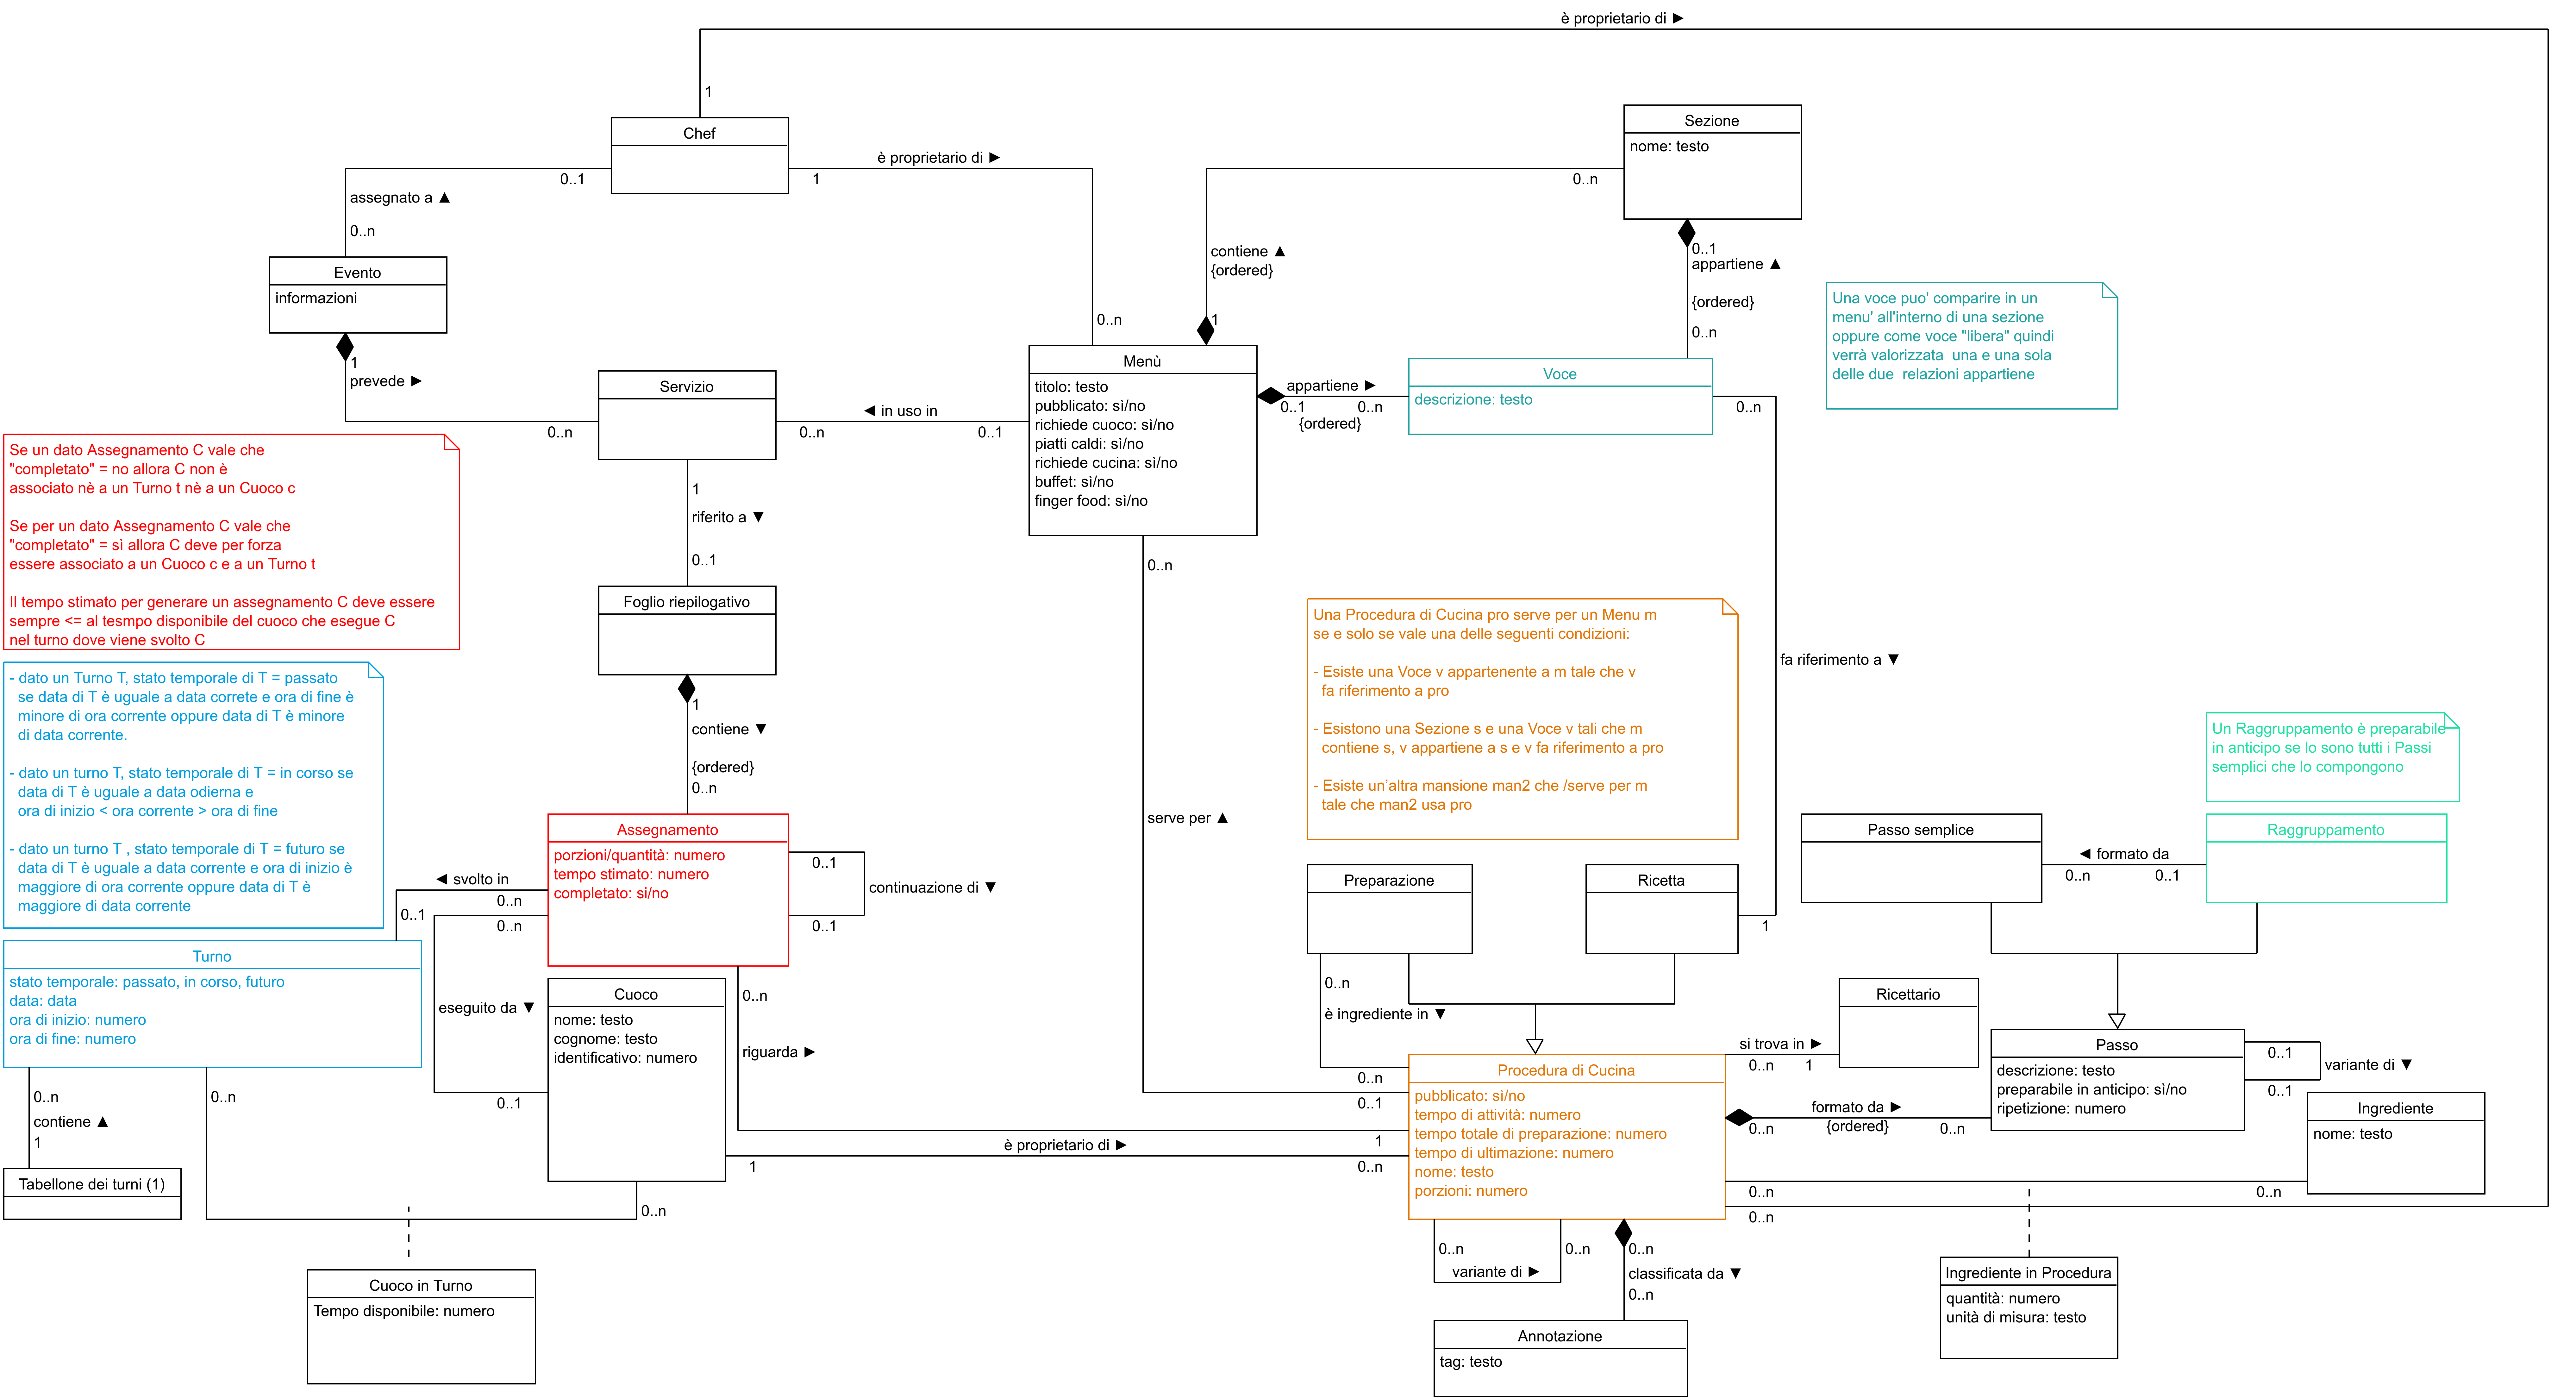
\includegraphics[width=\textwidth]{../resources/img/Domain Model.png}
\end{figure}
\normalpapersize

\chapter{Diagrammi di Sequenza di Sistema}
\centering
\section*{Scenario Principale di Successo}\addcontentsline{toc}{section}{Scenario Principale di Successo}
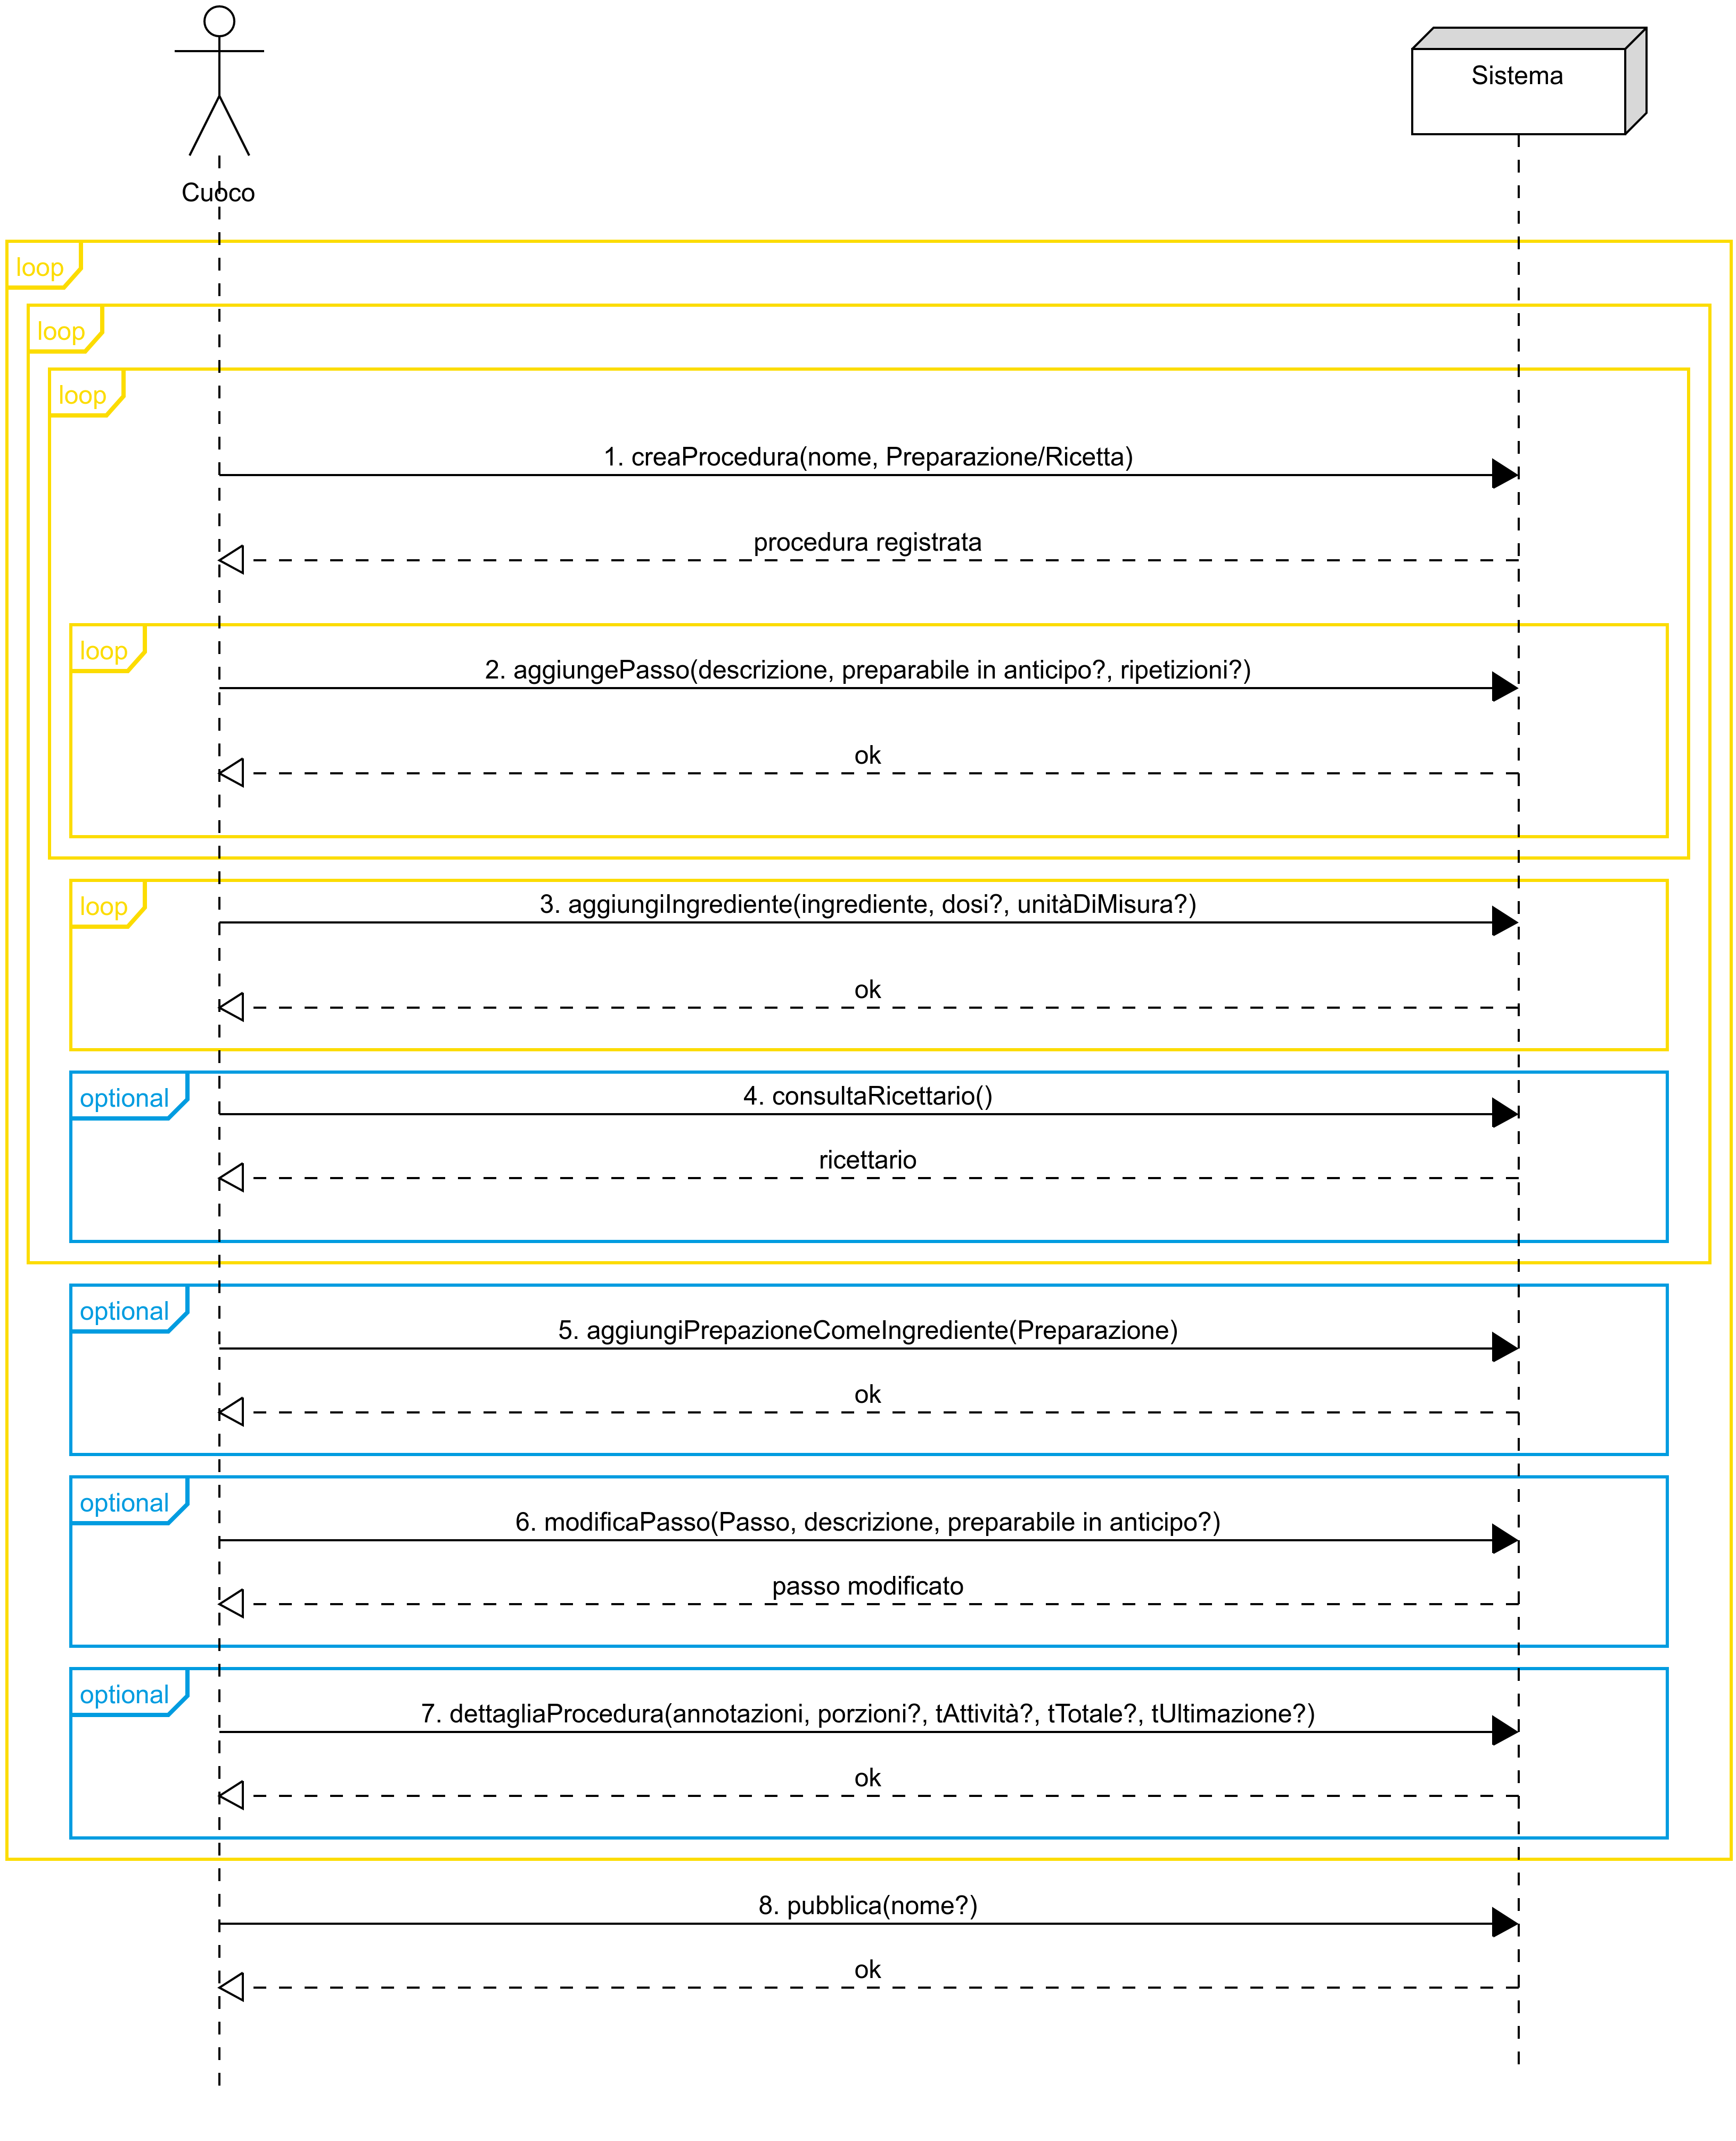
\includegraphics[max width=\textwidth, max height=158mm]{../resources/img/GRP/SSD/main.png}

\section*{Estensioni 1}\addcontentsline{toc}{subsection}{Estensioni 1}
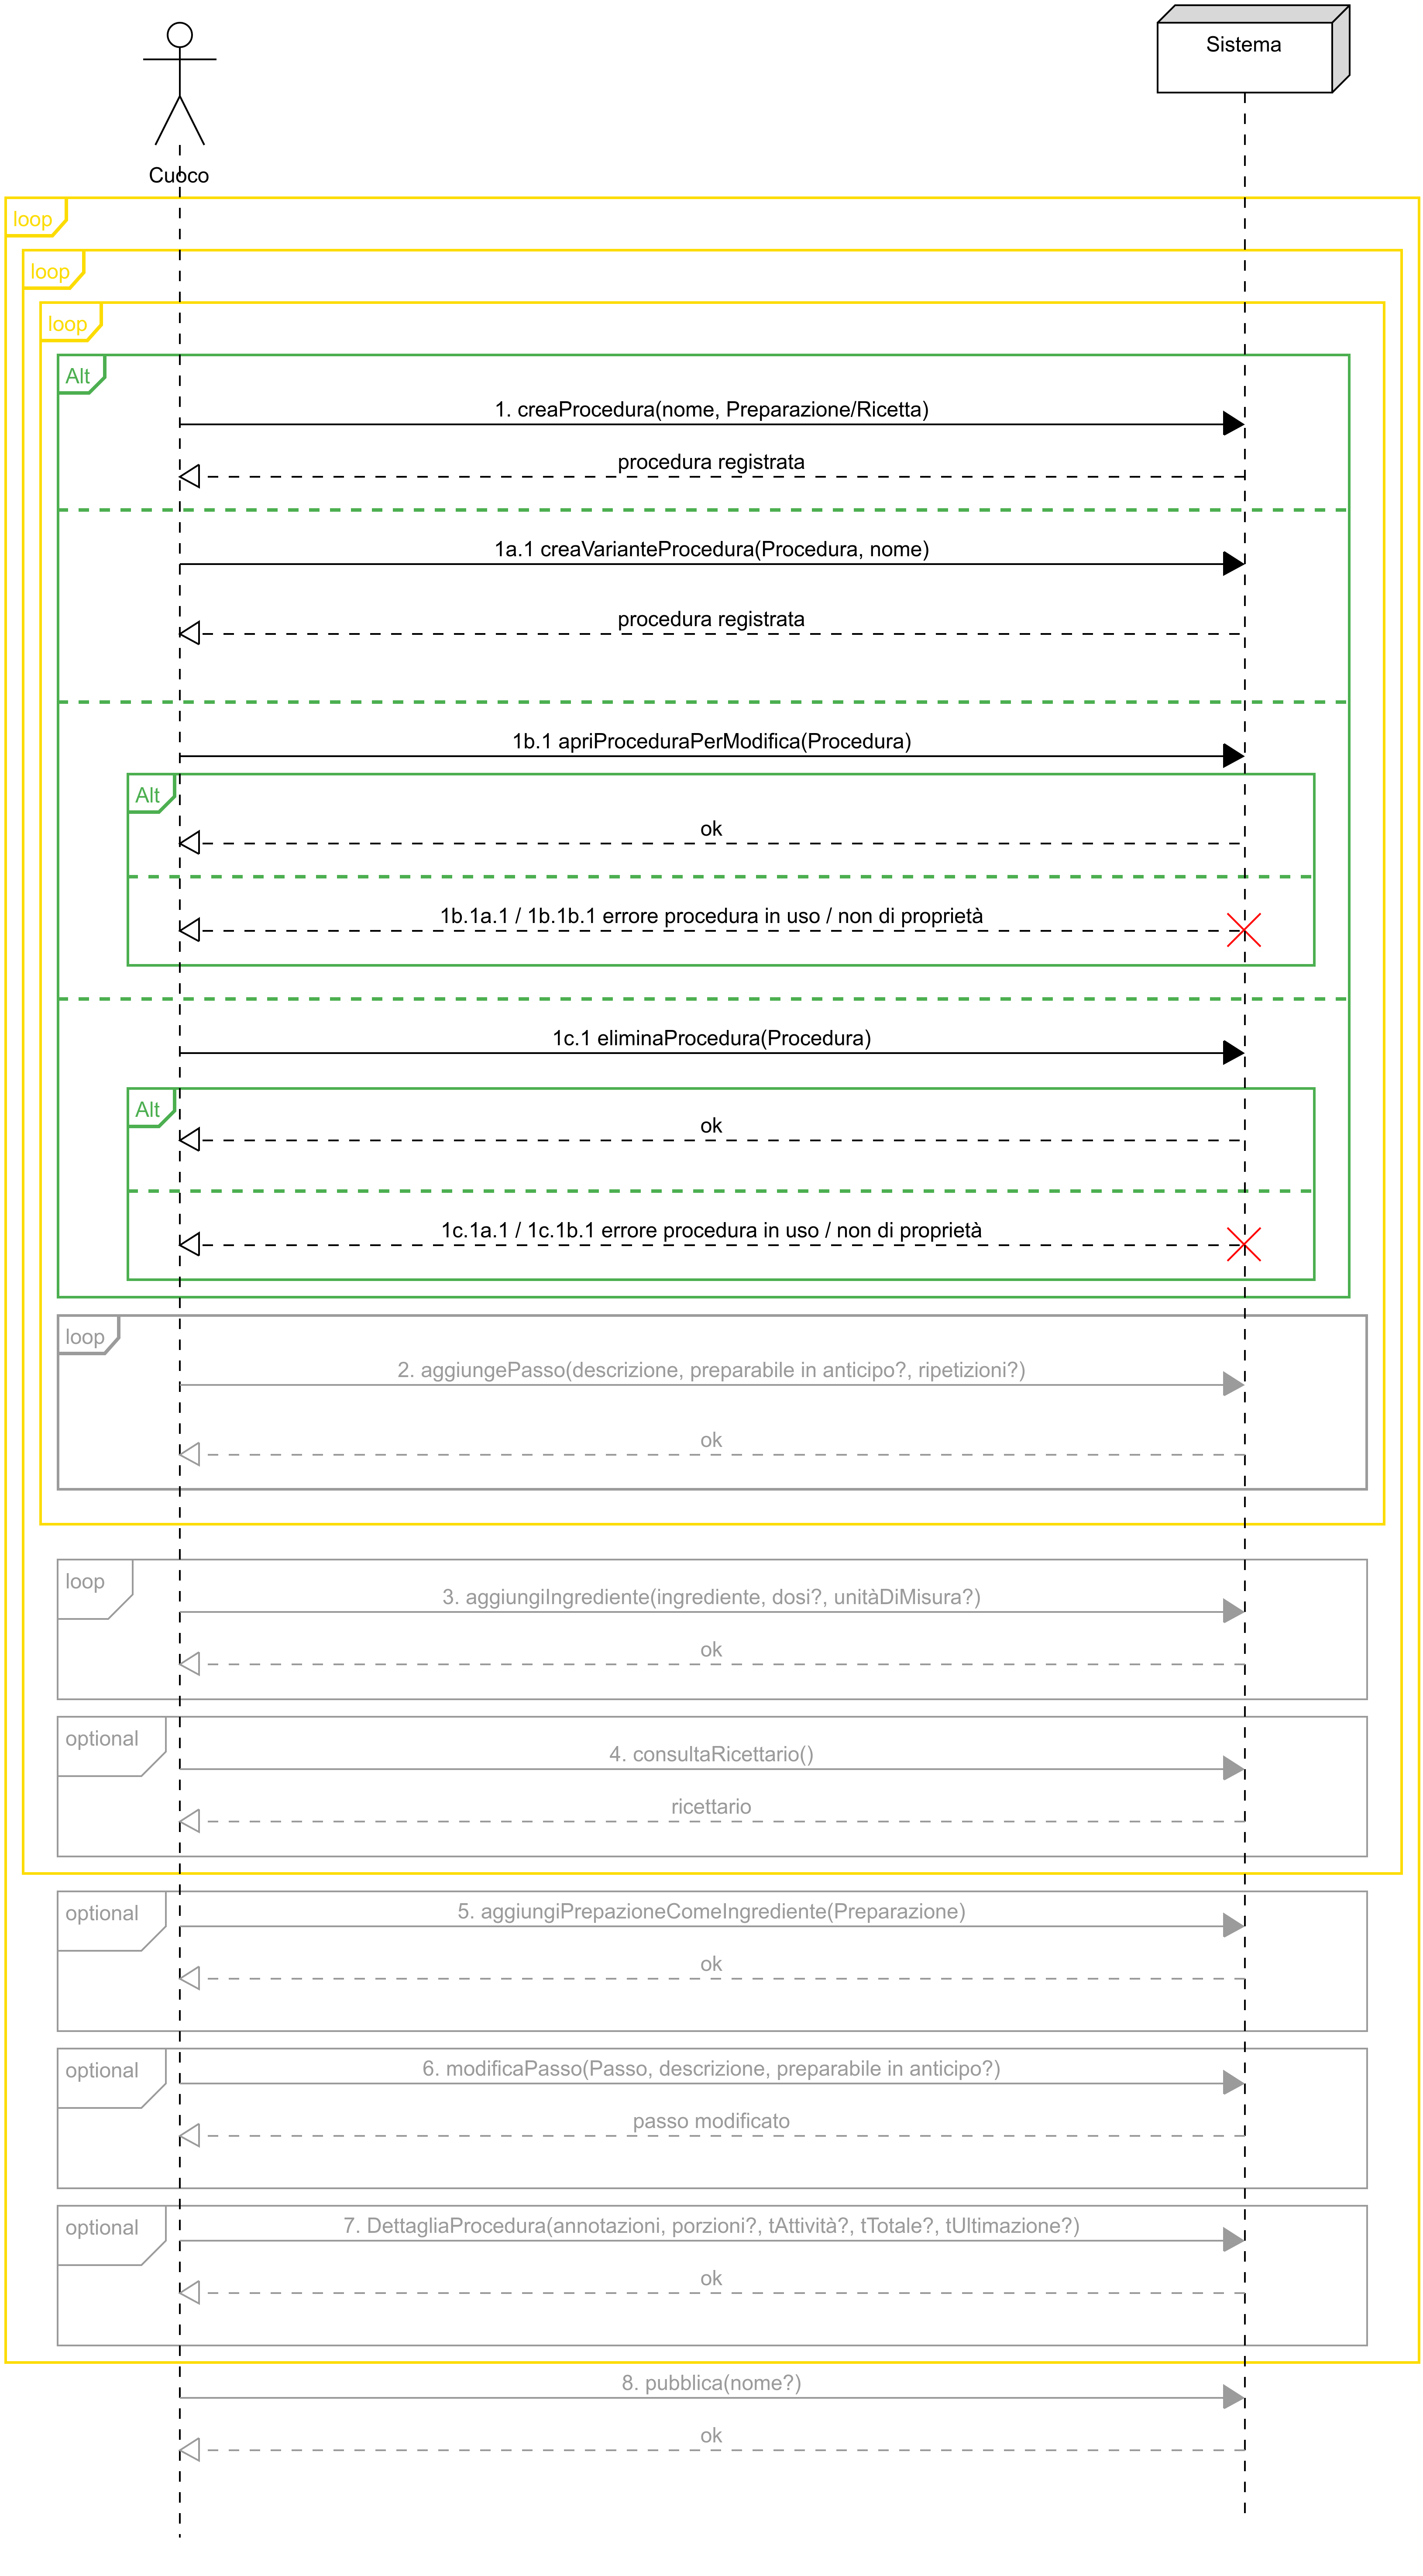
\includegraphics[max width=\textwidth, max height=190mm]{../resources/img/GRP/SSD/ext1.png}

\section*{Estensioni 2}\addcontentsline{toc}{subsection}{Estensioni 2}
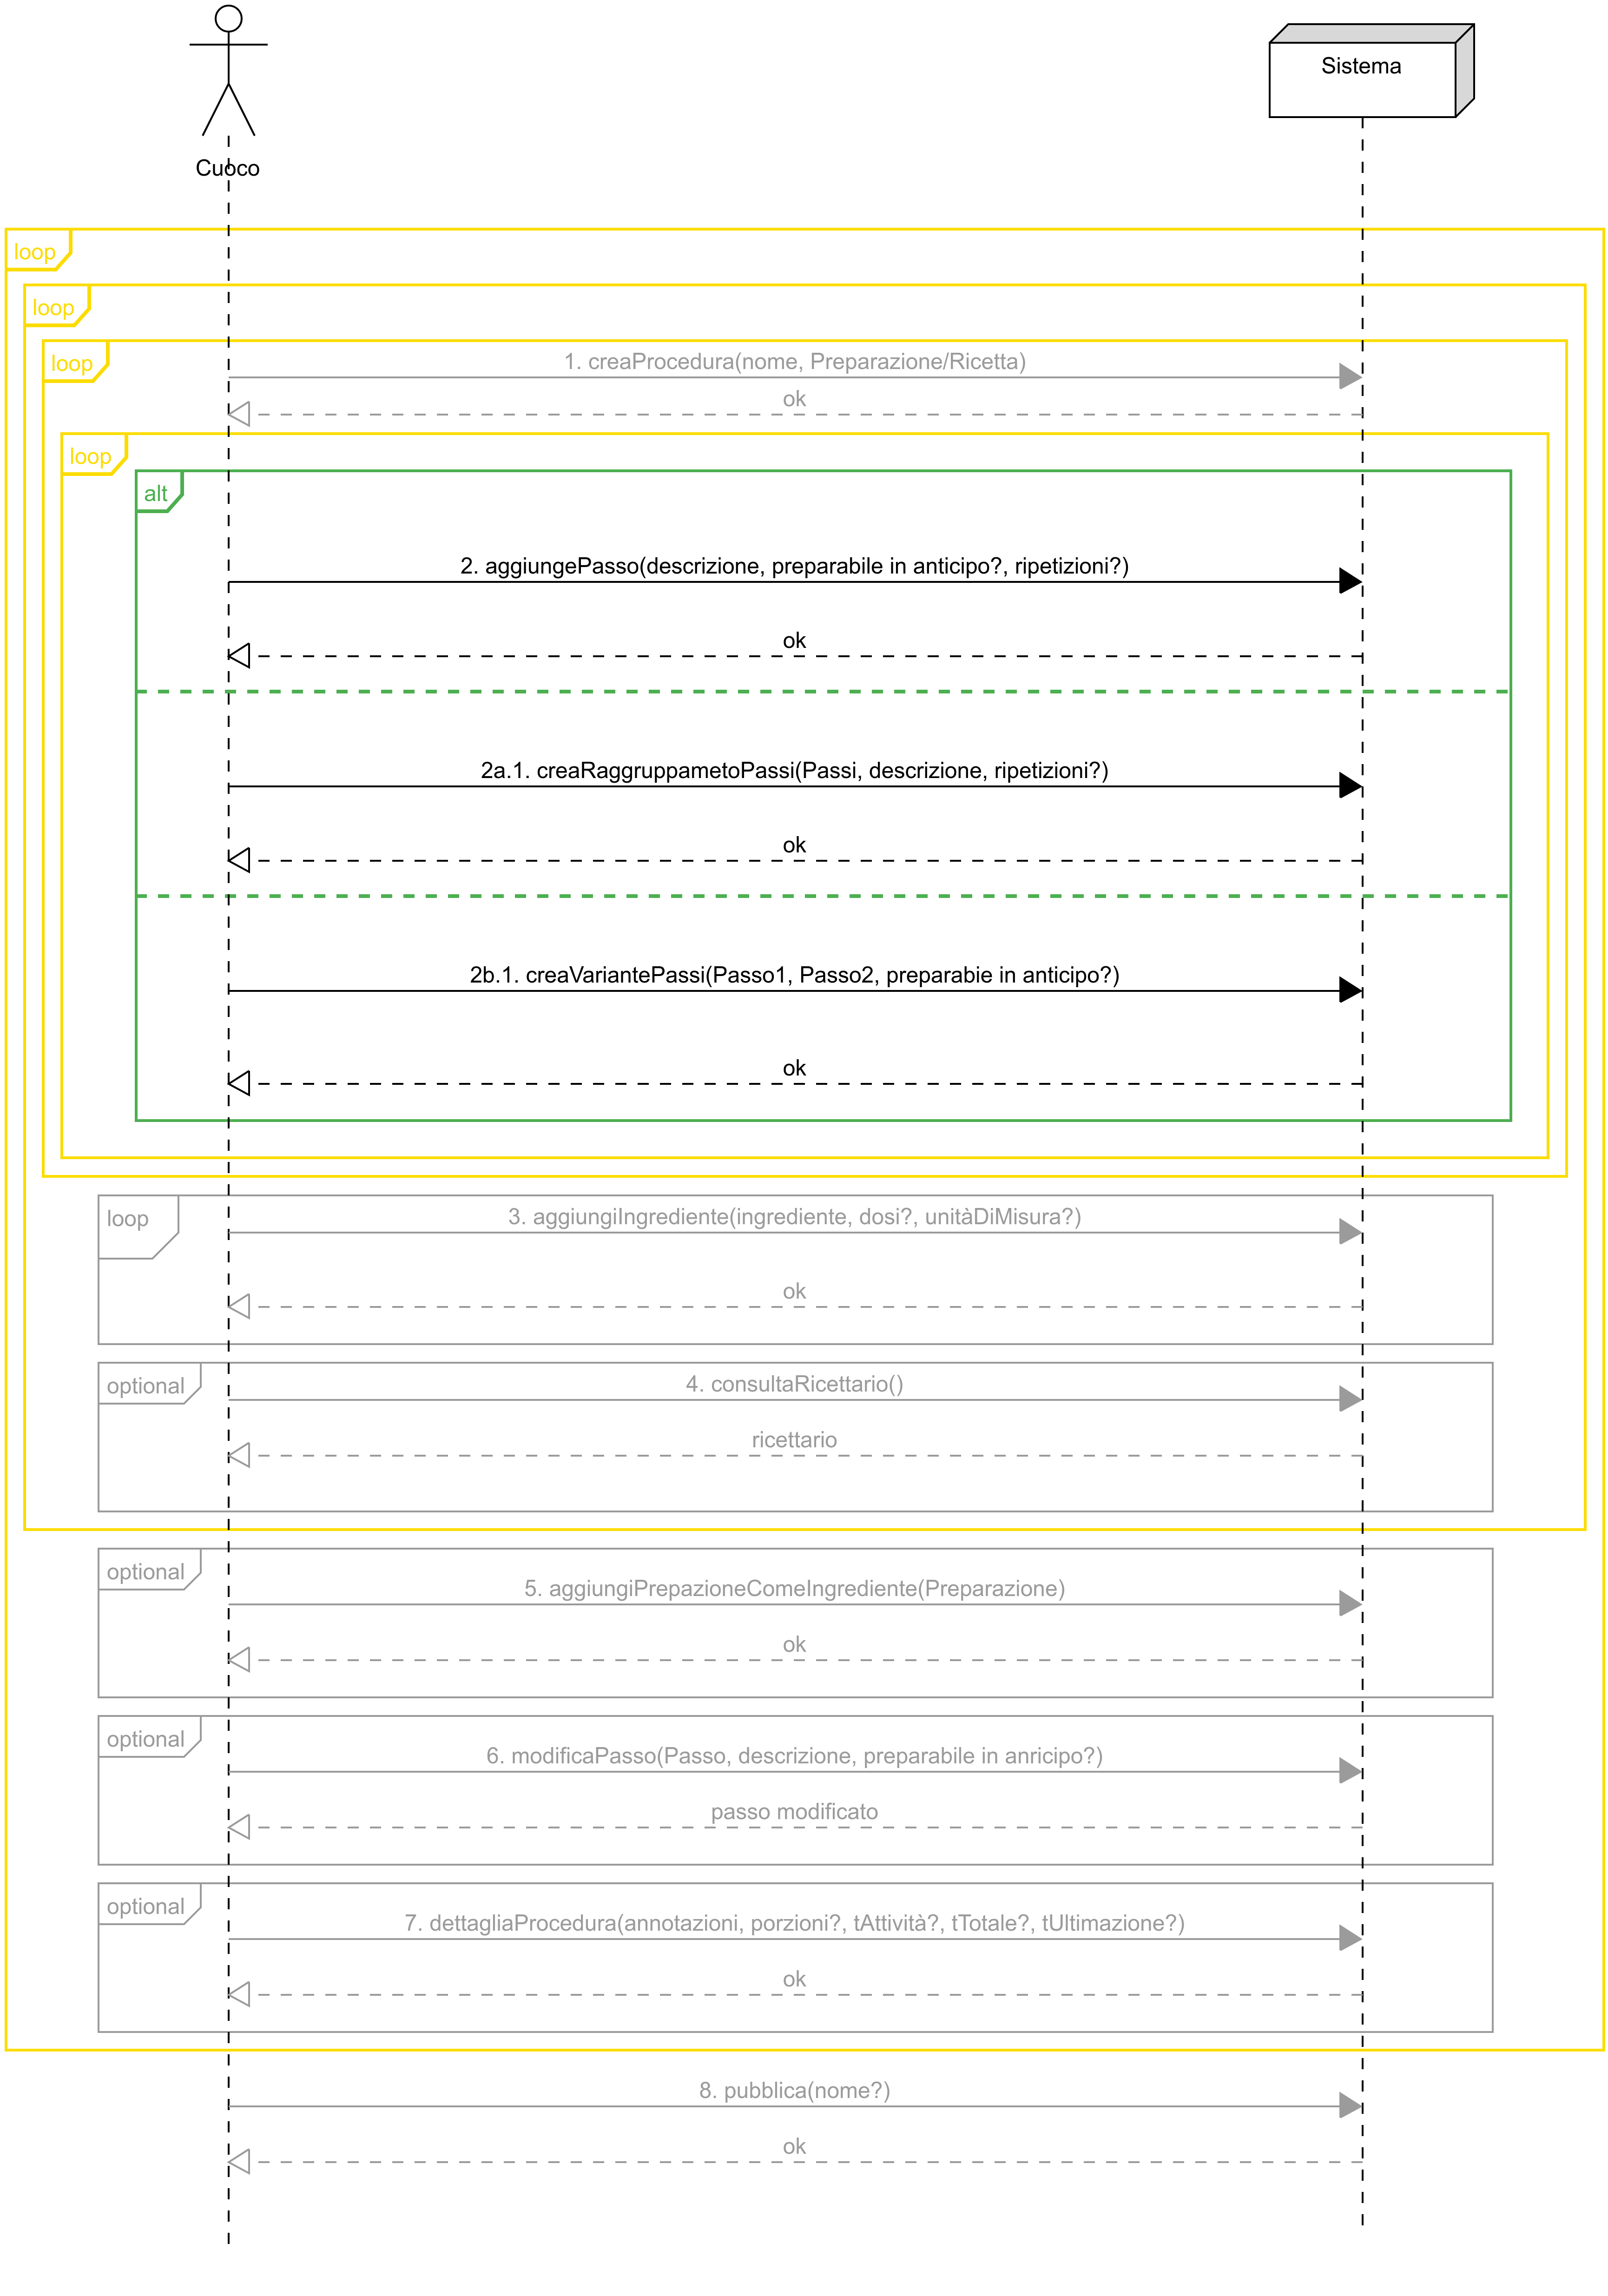
\includegraphics[max width=\textwidth, max height=190mm]{../resources/img/GRP/SSD/ext2.png}

\section*{Estensioni 3}\addcontentsline{toc}{subsection}{Estensioni 3}
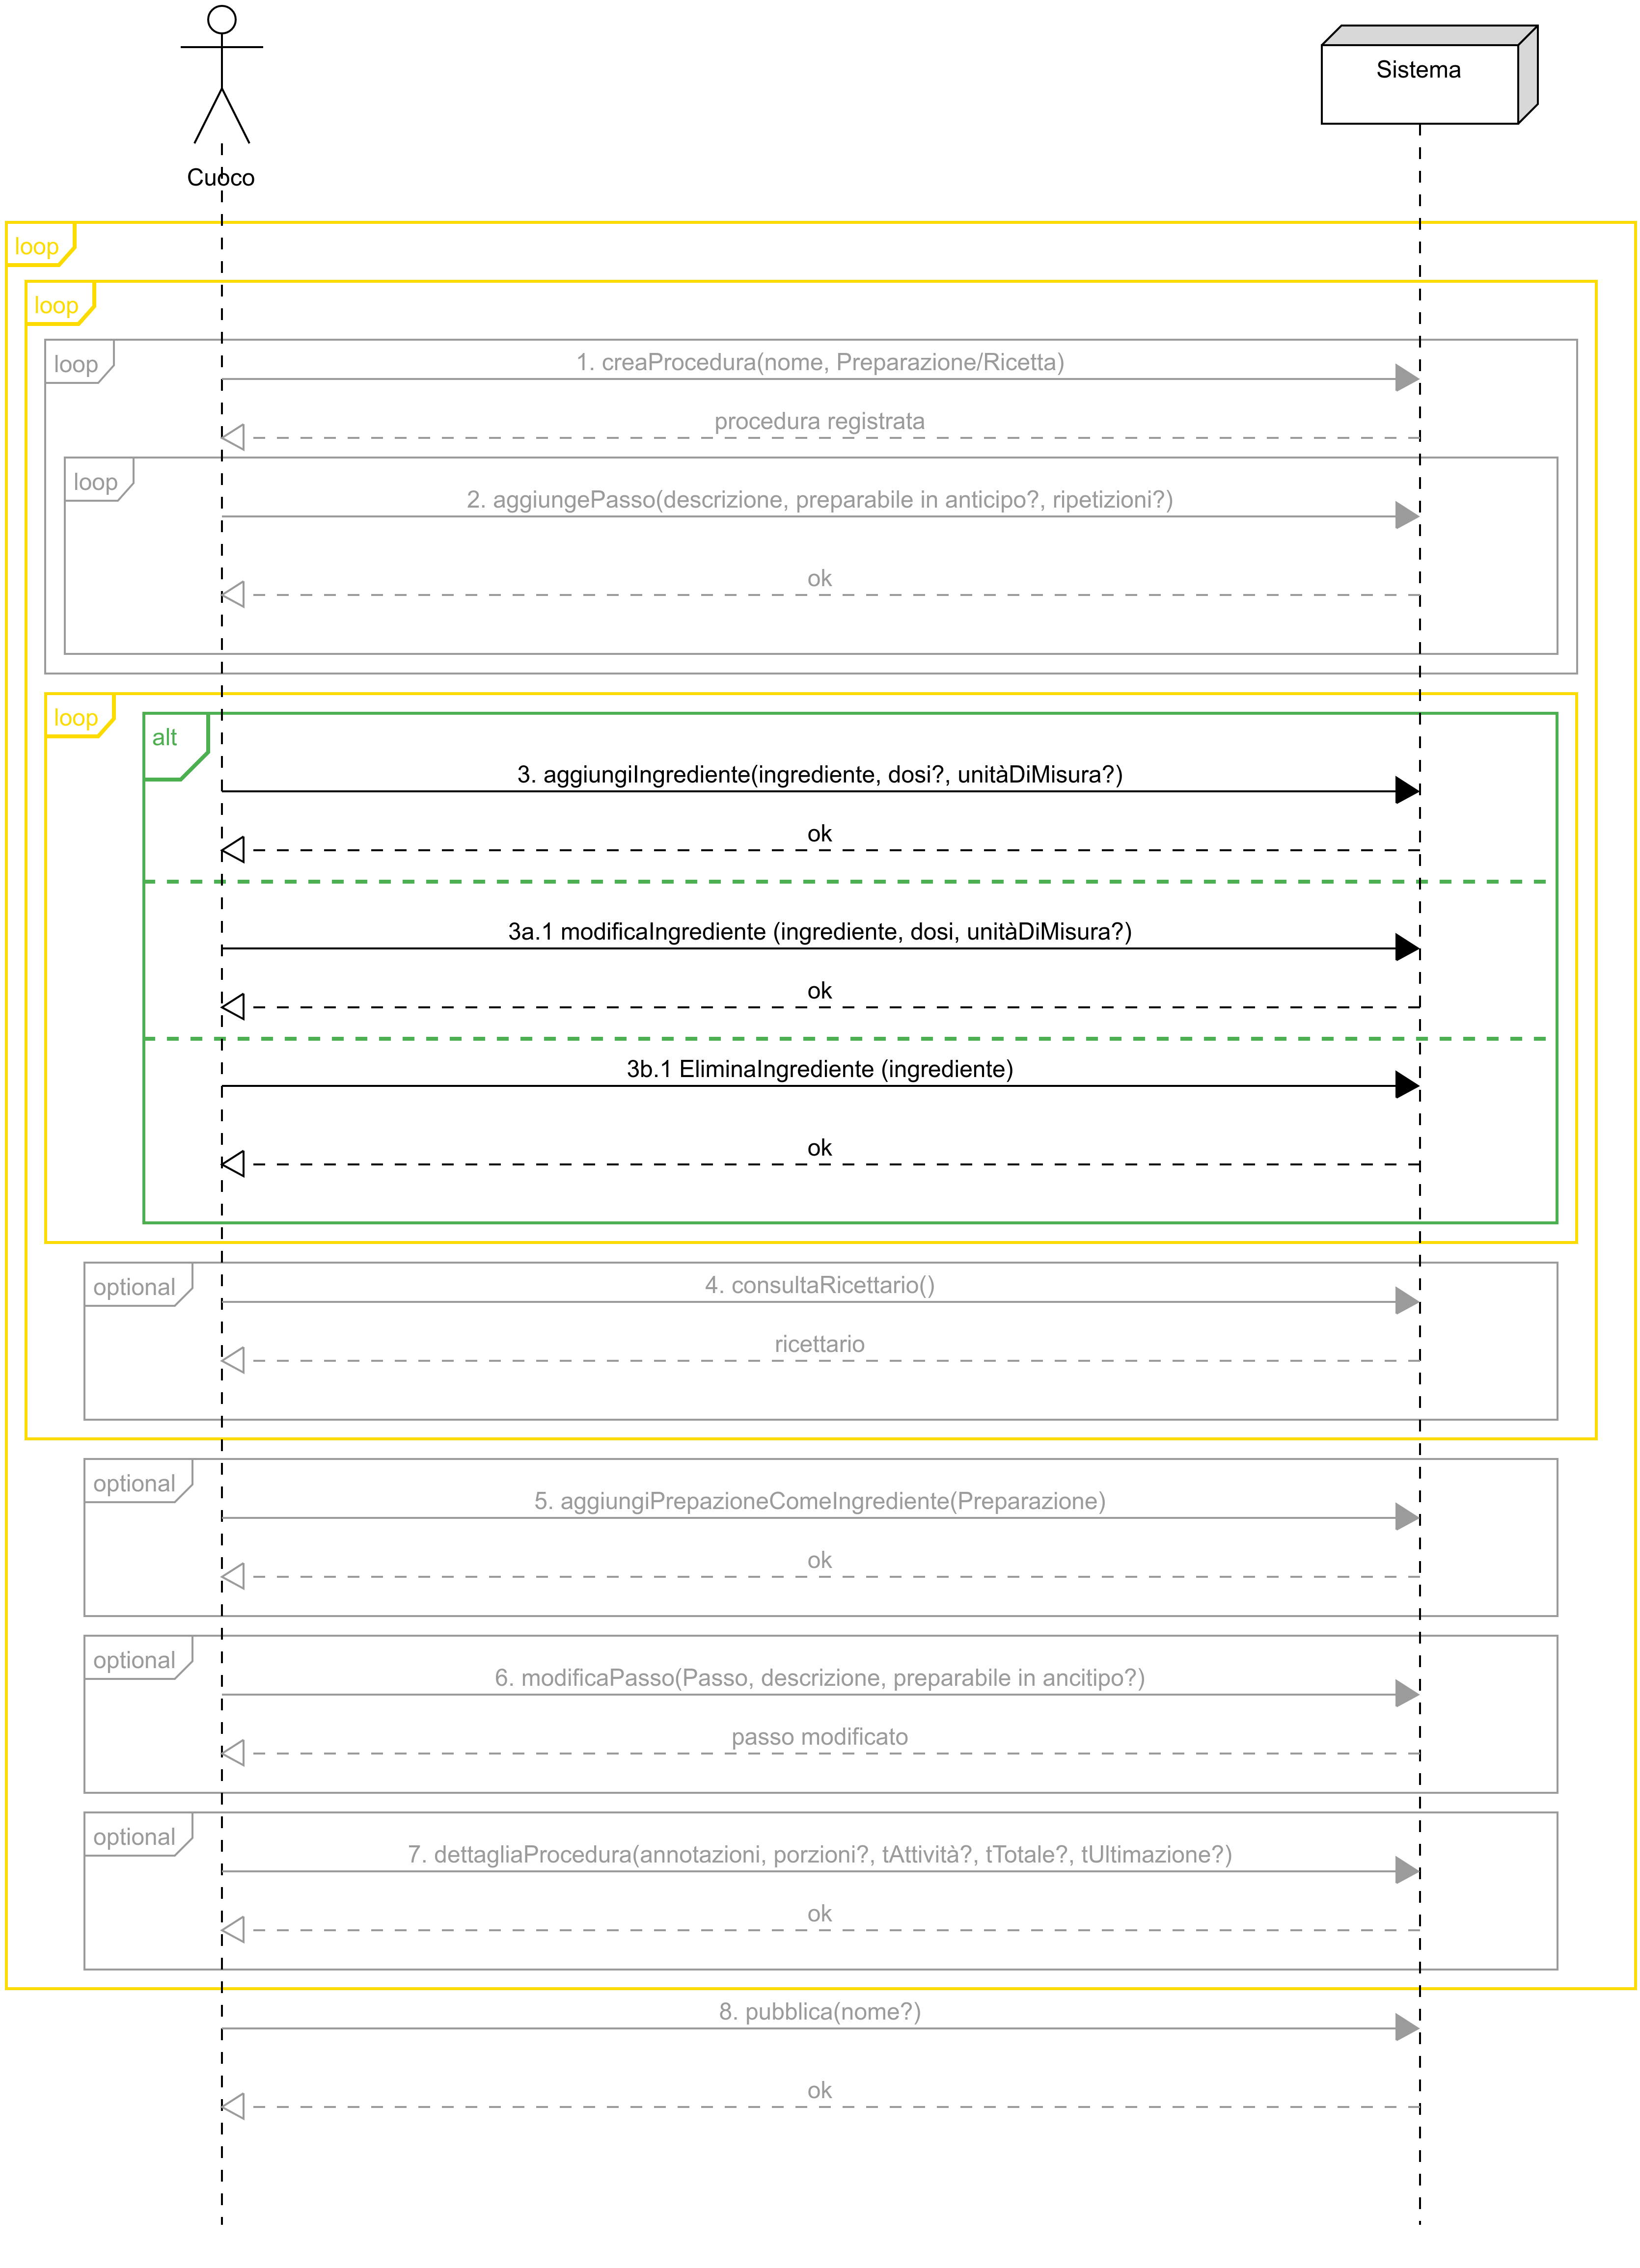
\includegraphics[max width=\textwidth, max height=190mm]{../resources/img/GRP/SSD/ext3.png}

\section*{Estensioni 5}\addcontentsline{toc}{subsection}{Estensioni 5}
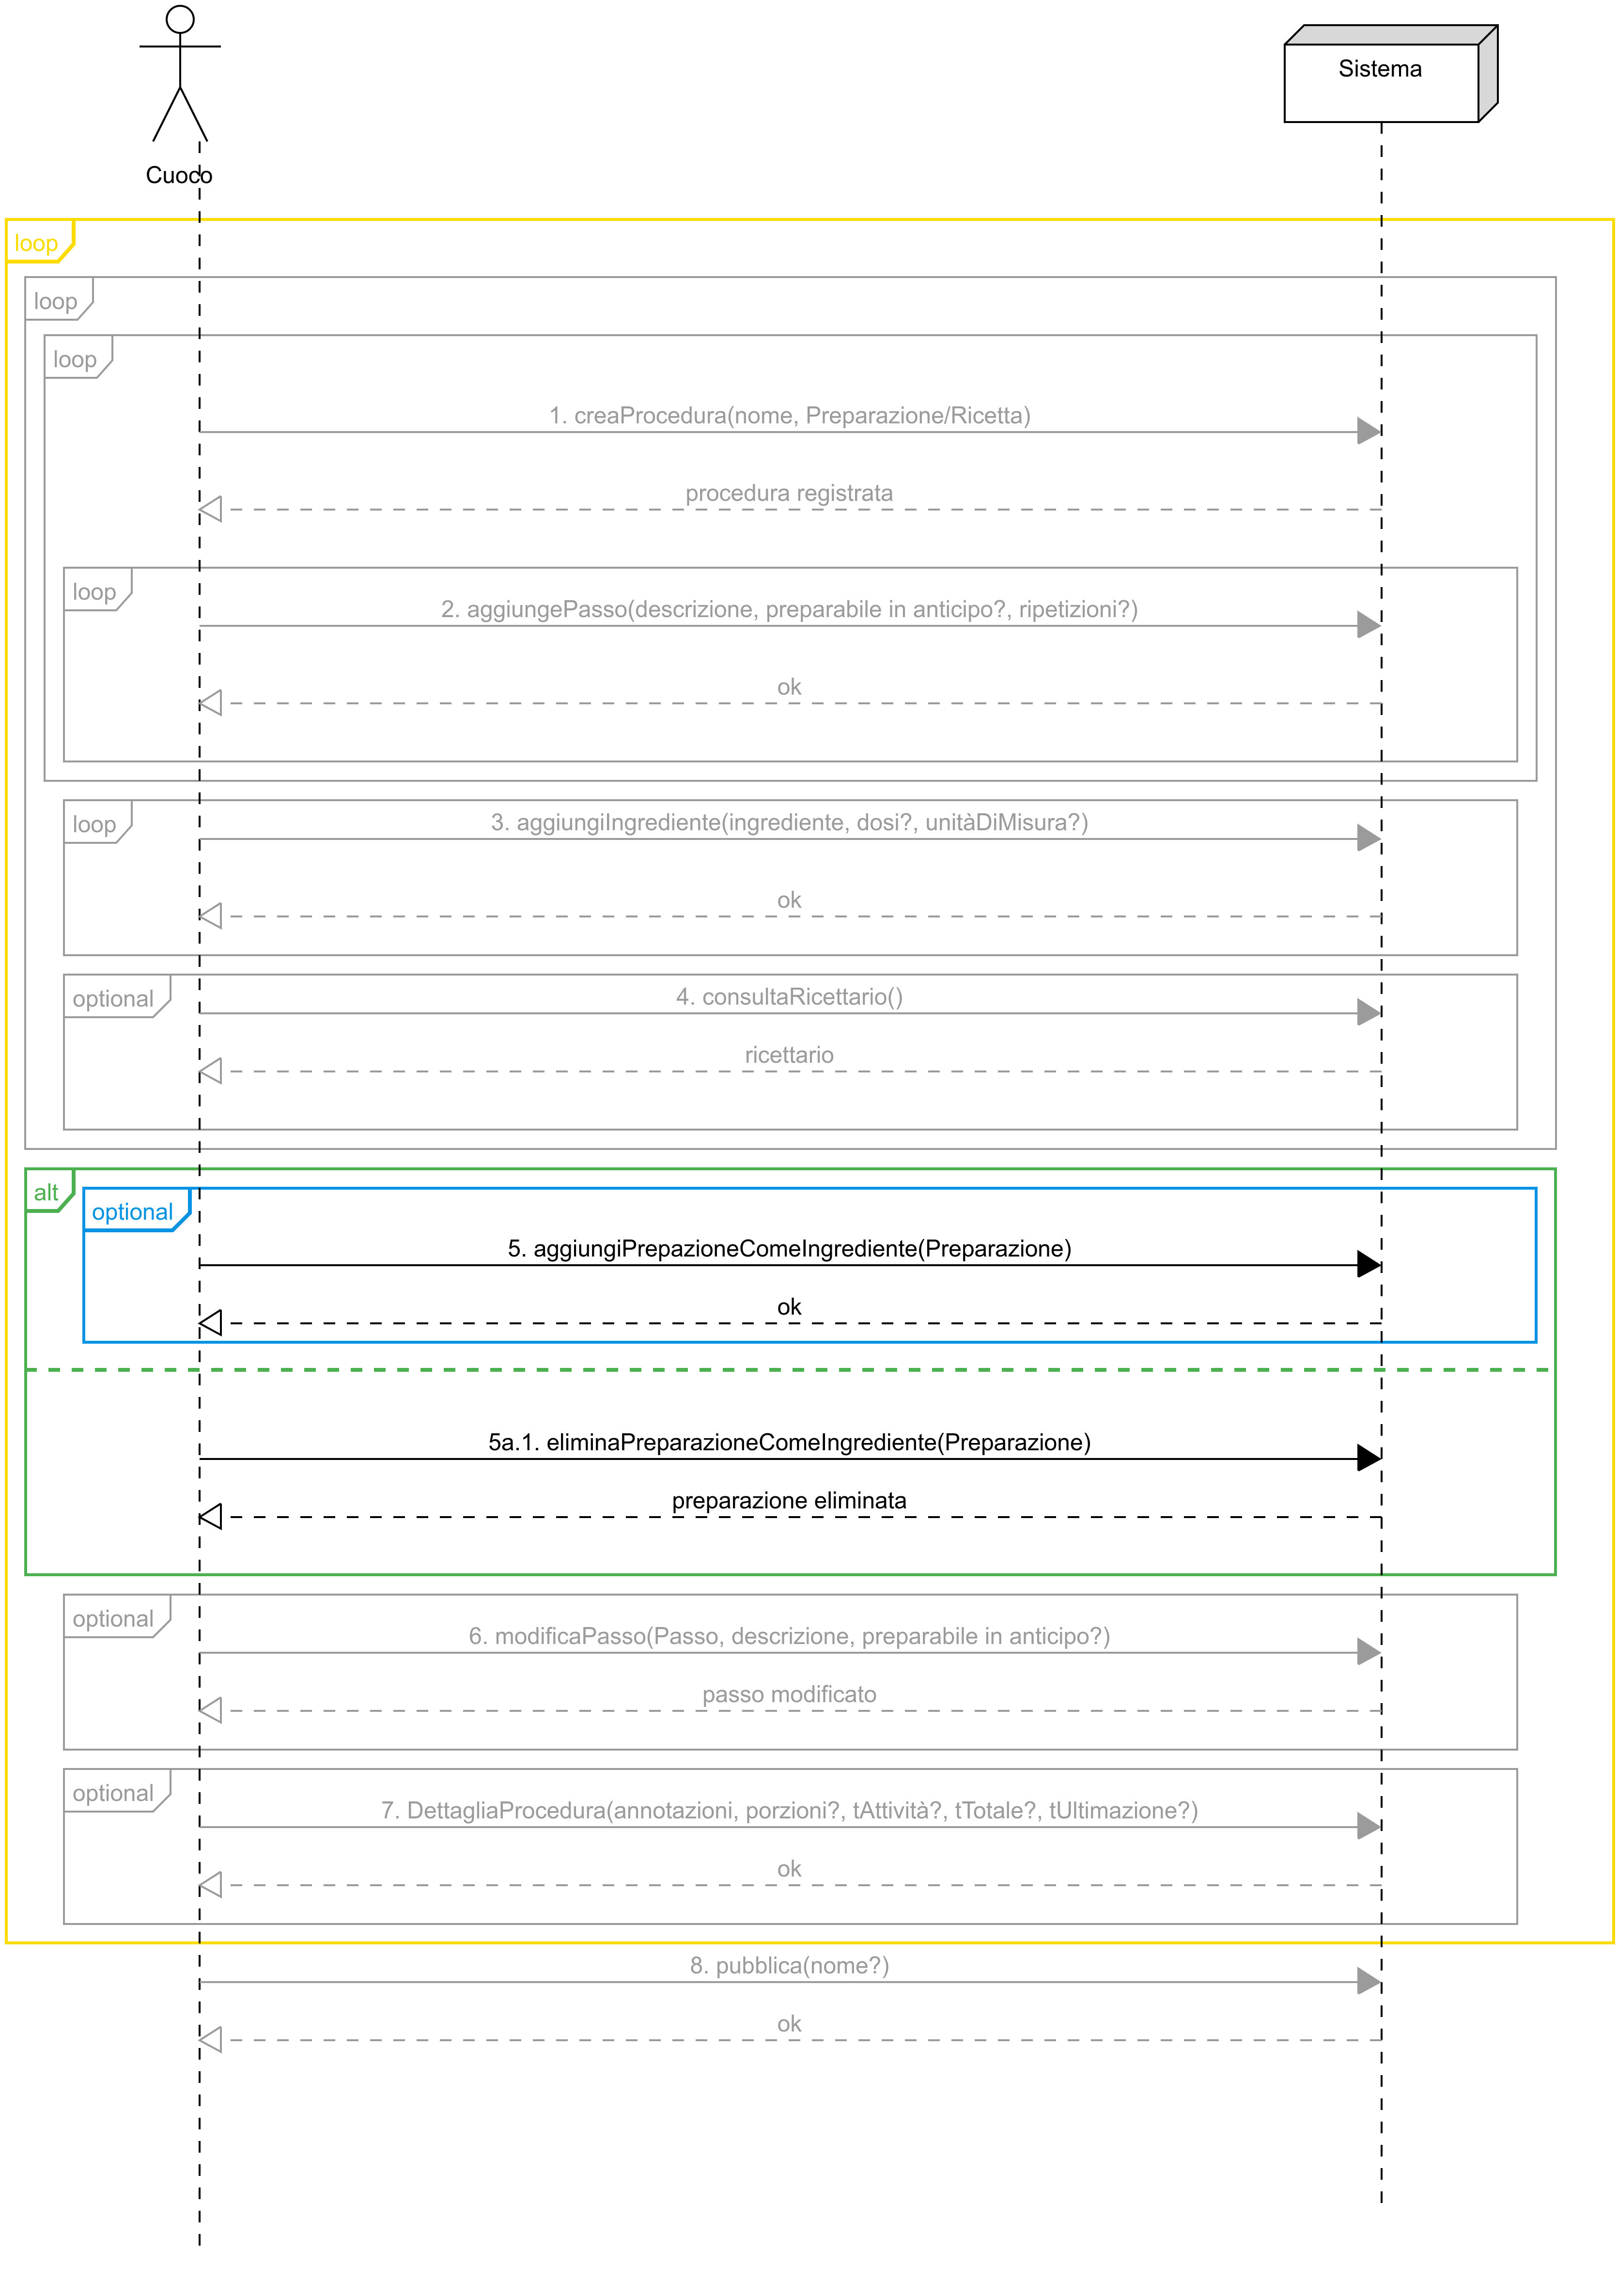
\includegraphics[max width=\textwidth, max height=190mm]{../resources/img/GRP/SSD/ext5.png}

\section*{Estensioni 6}\addcontentsline{toc}{subsection}{Estensioni 6}
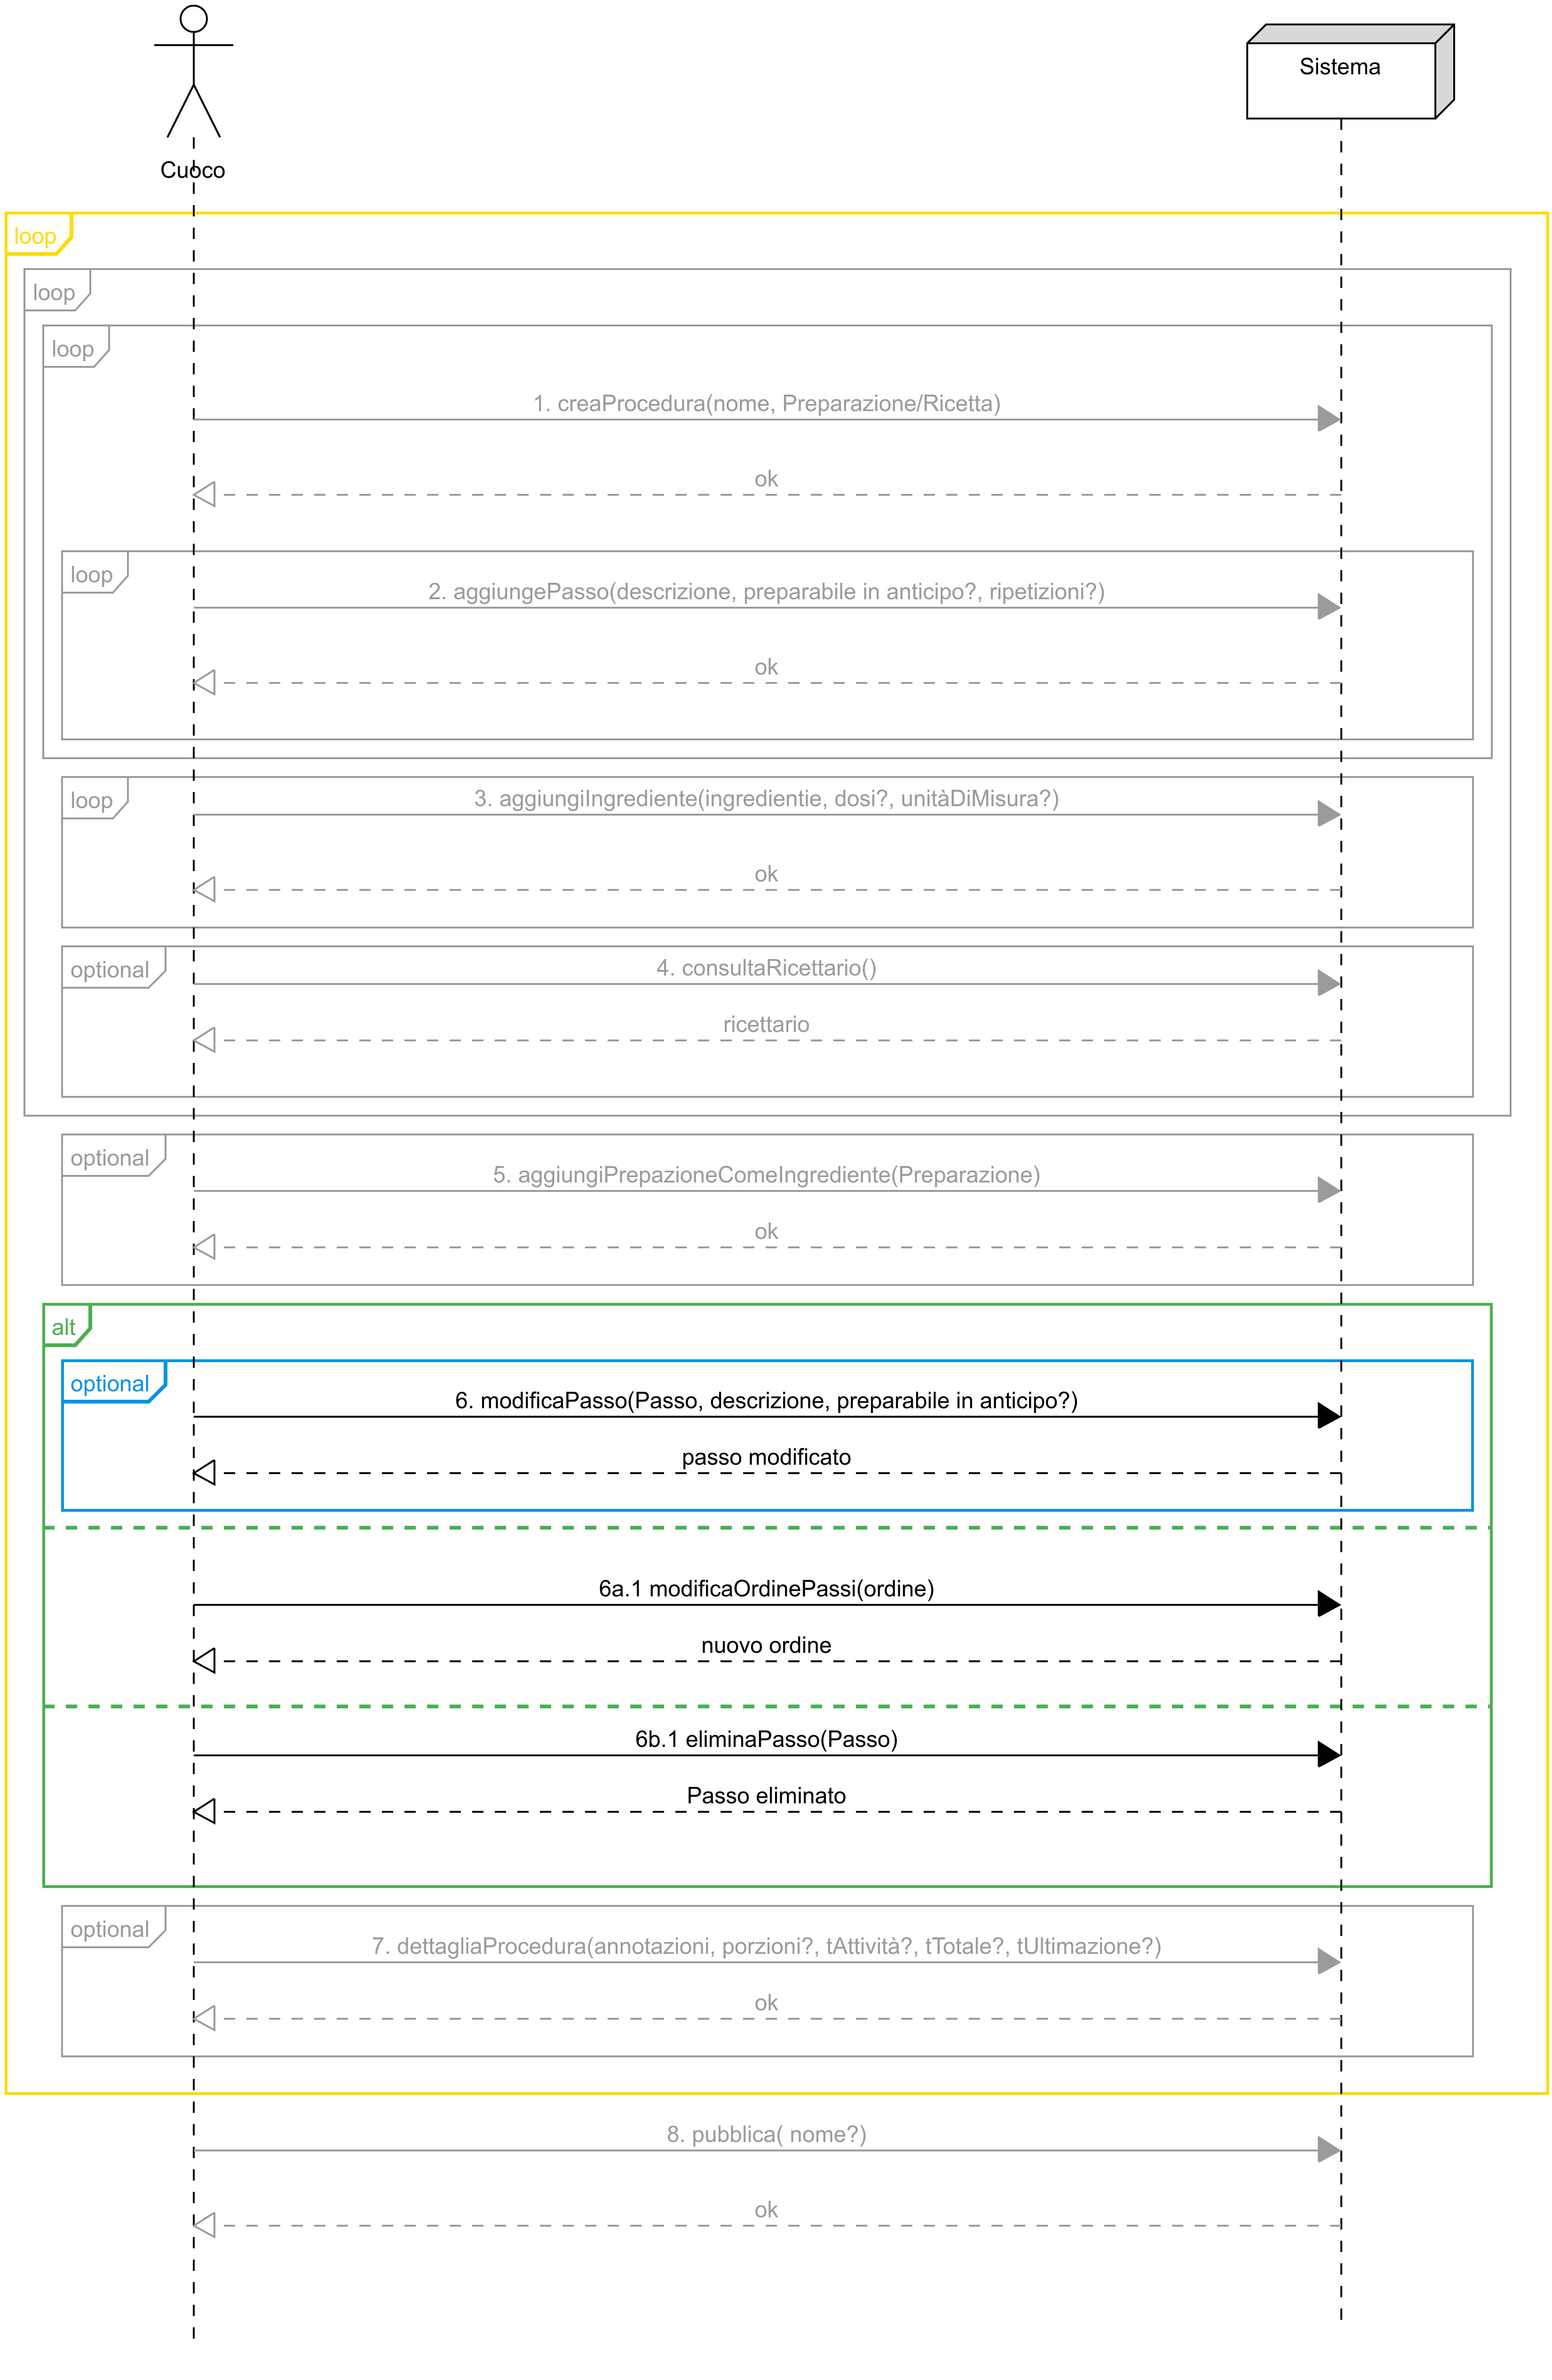
\includegraphics[max width=\textwidth, max height=190mm]{../resources/img/GRP/SSD/ext6.png}

\section*{Estensioni 7}\addcontentsline{toc}{subsection}{Estensioni 7}
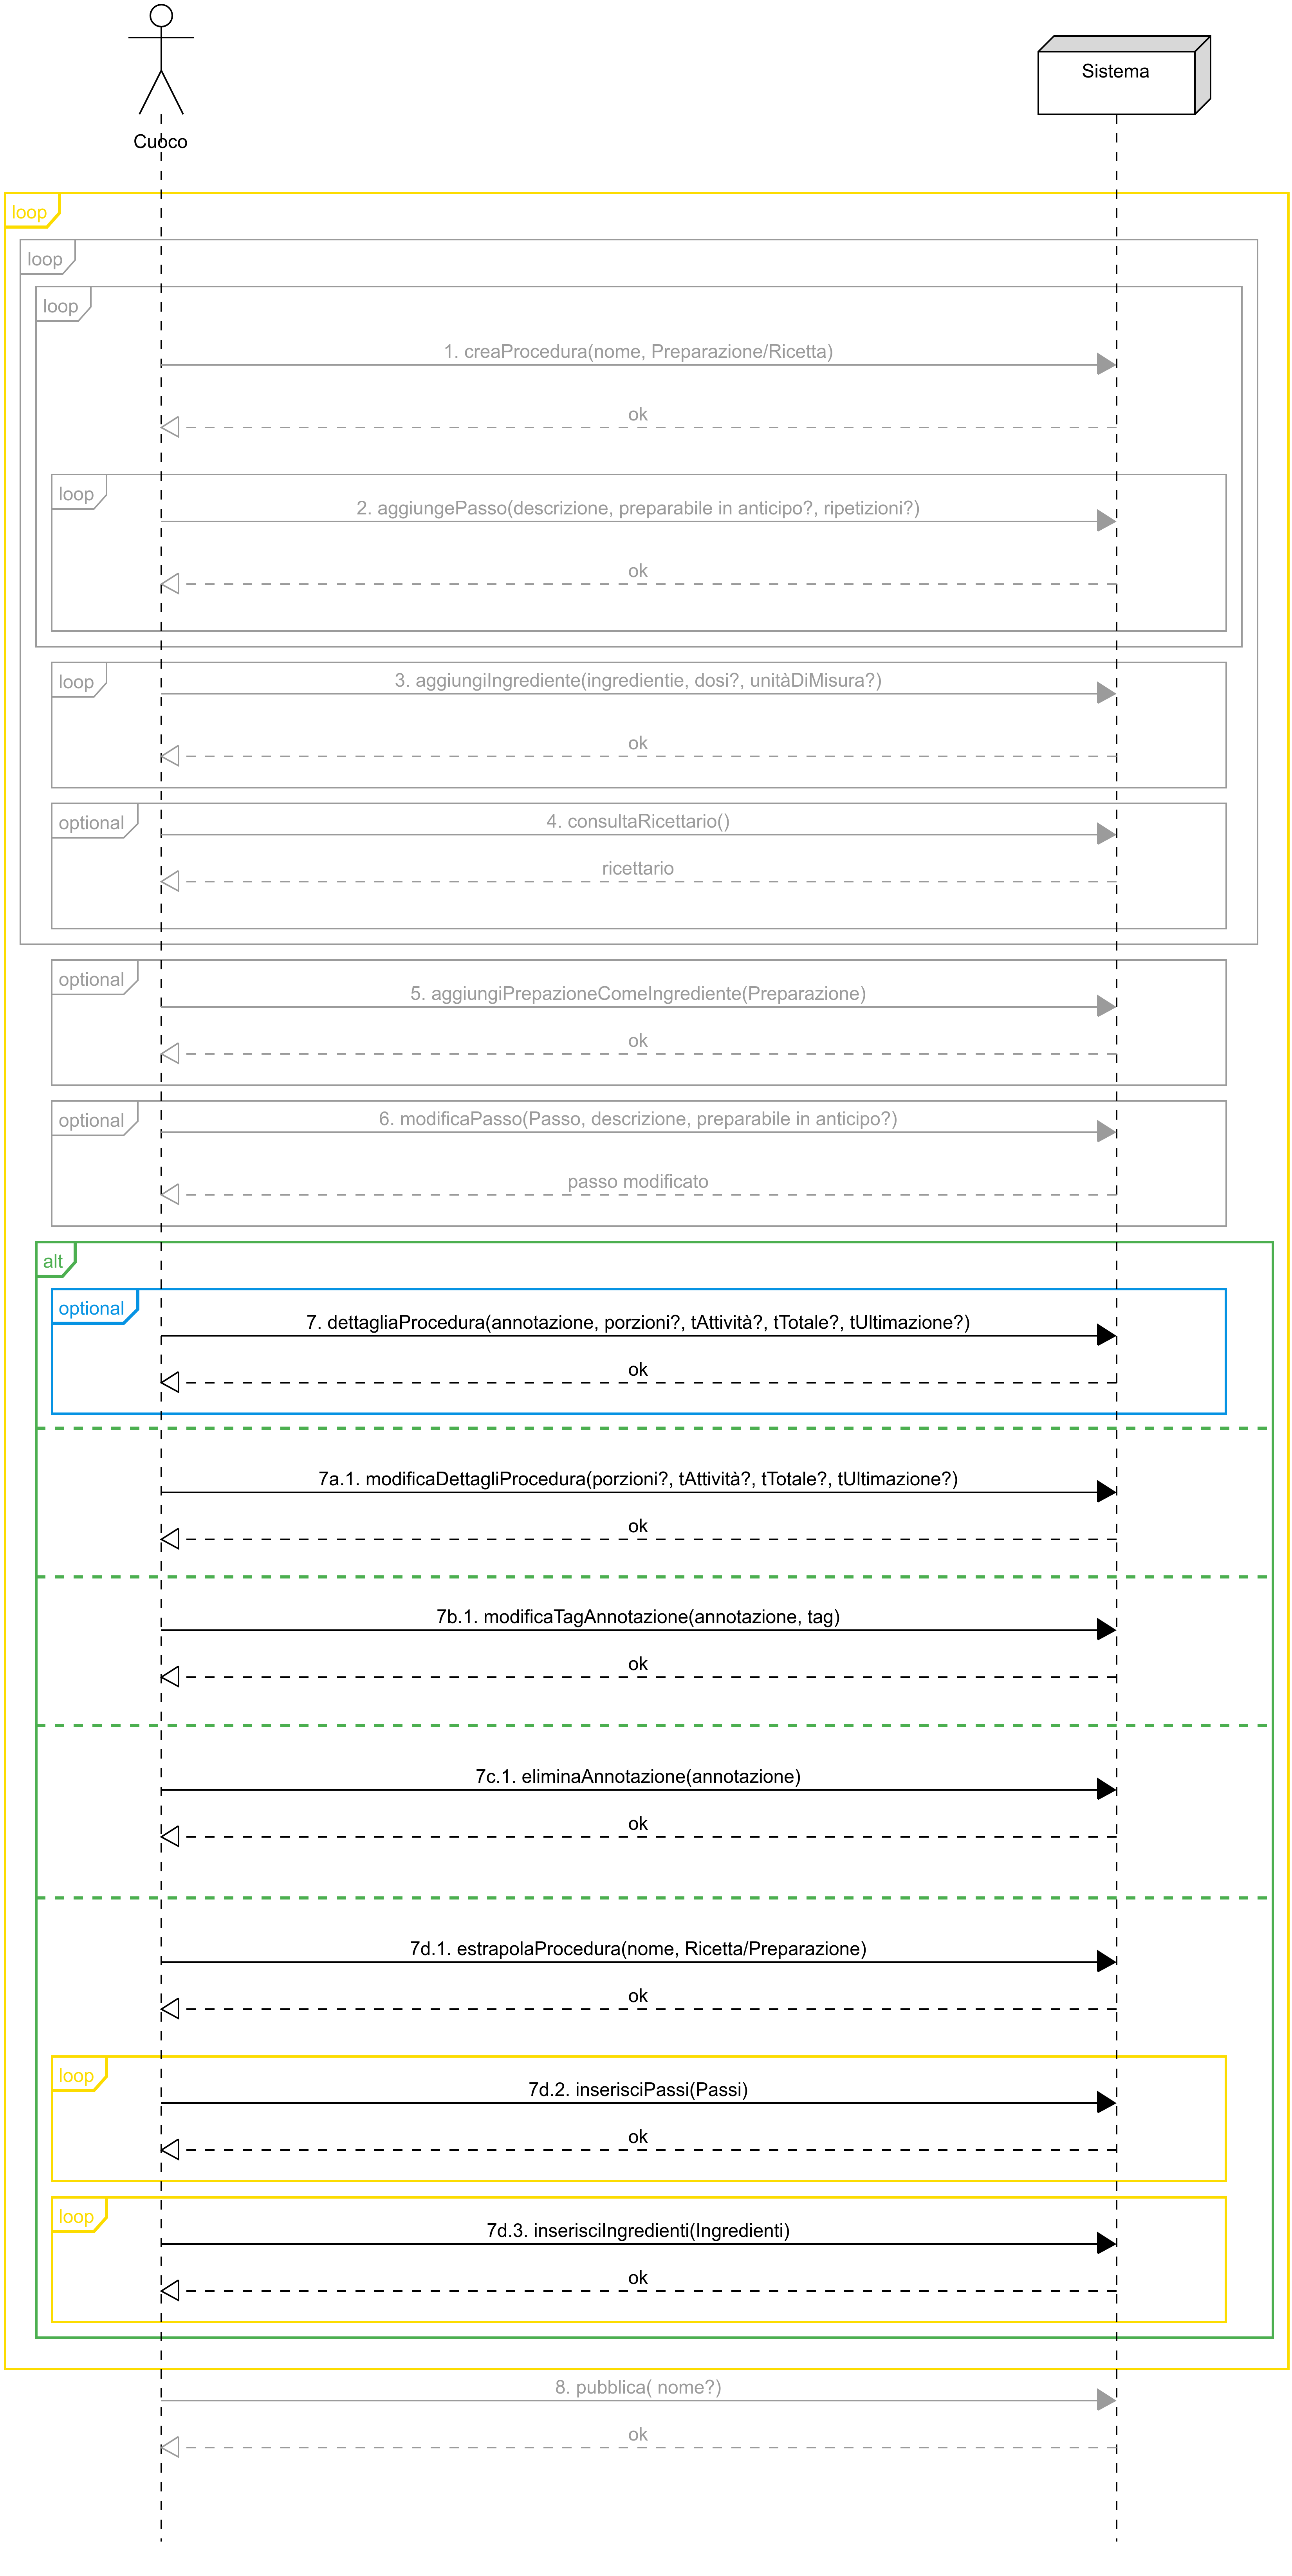
\includegraphics[max width=\textwidth, max height=190mm]{../resources/img/GRP/SSD/ext7.png}

\section*{Estensioni 8}\addcontentsline{toc}{subsection}{Estensioni 8}
\begin{figure}[H]
    \centering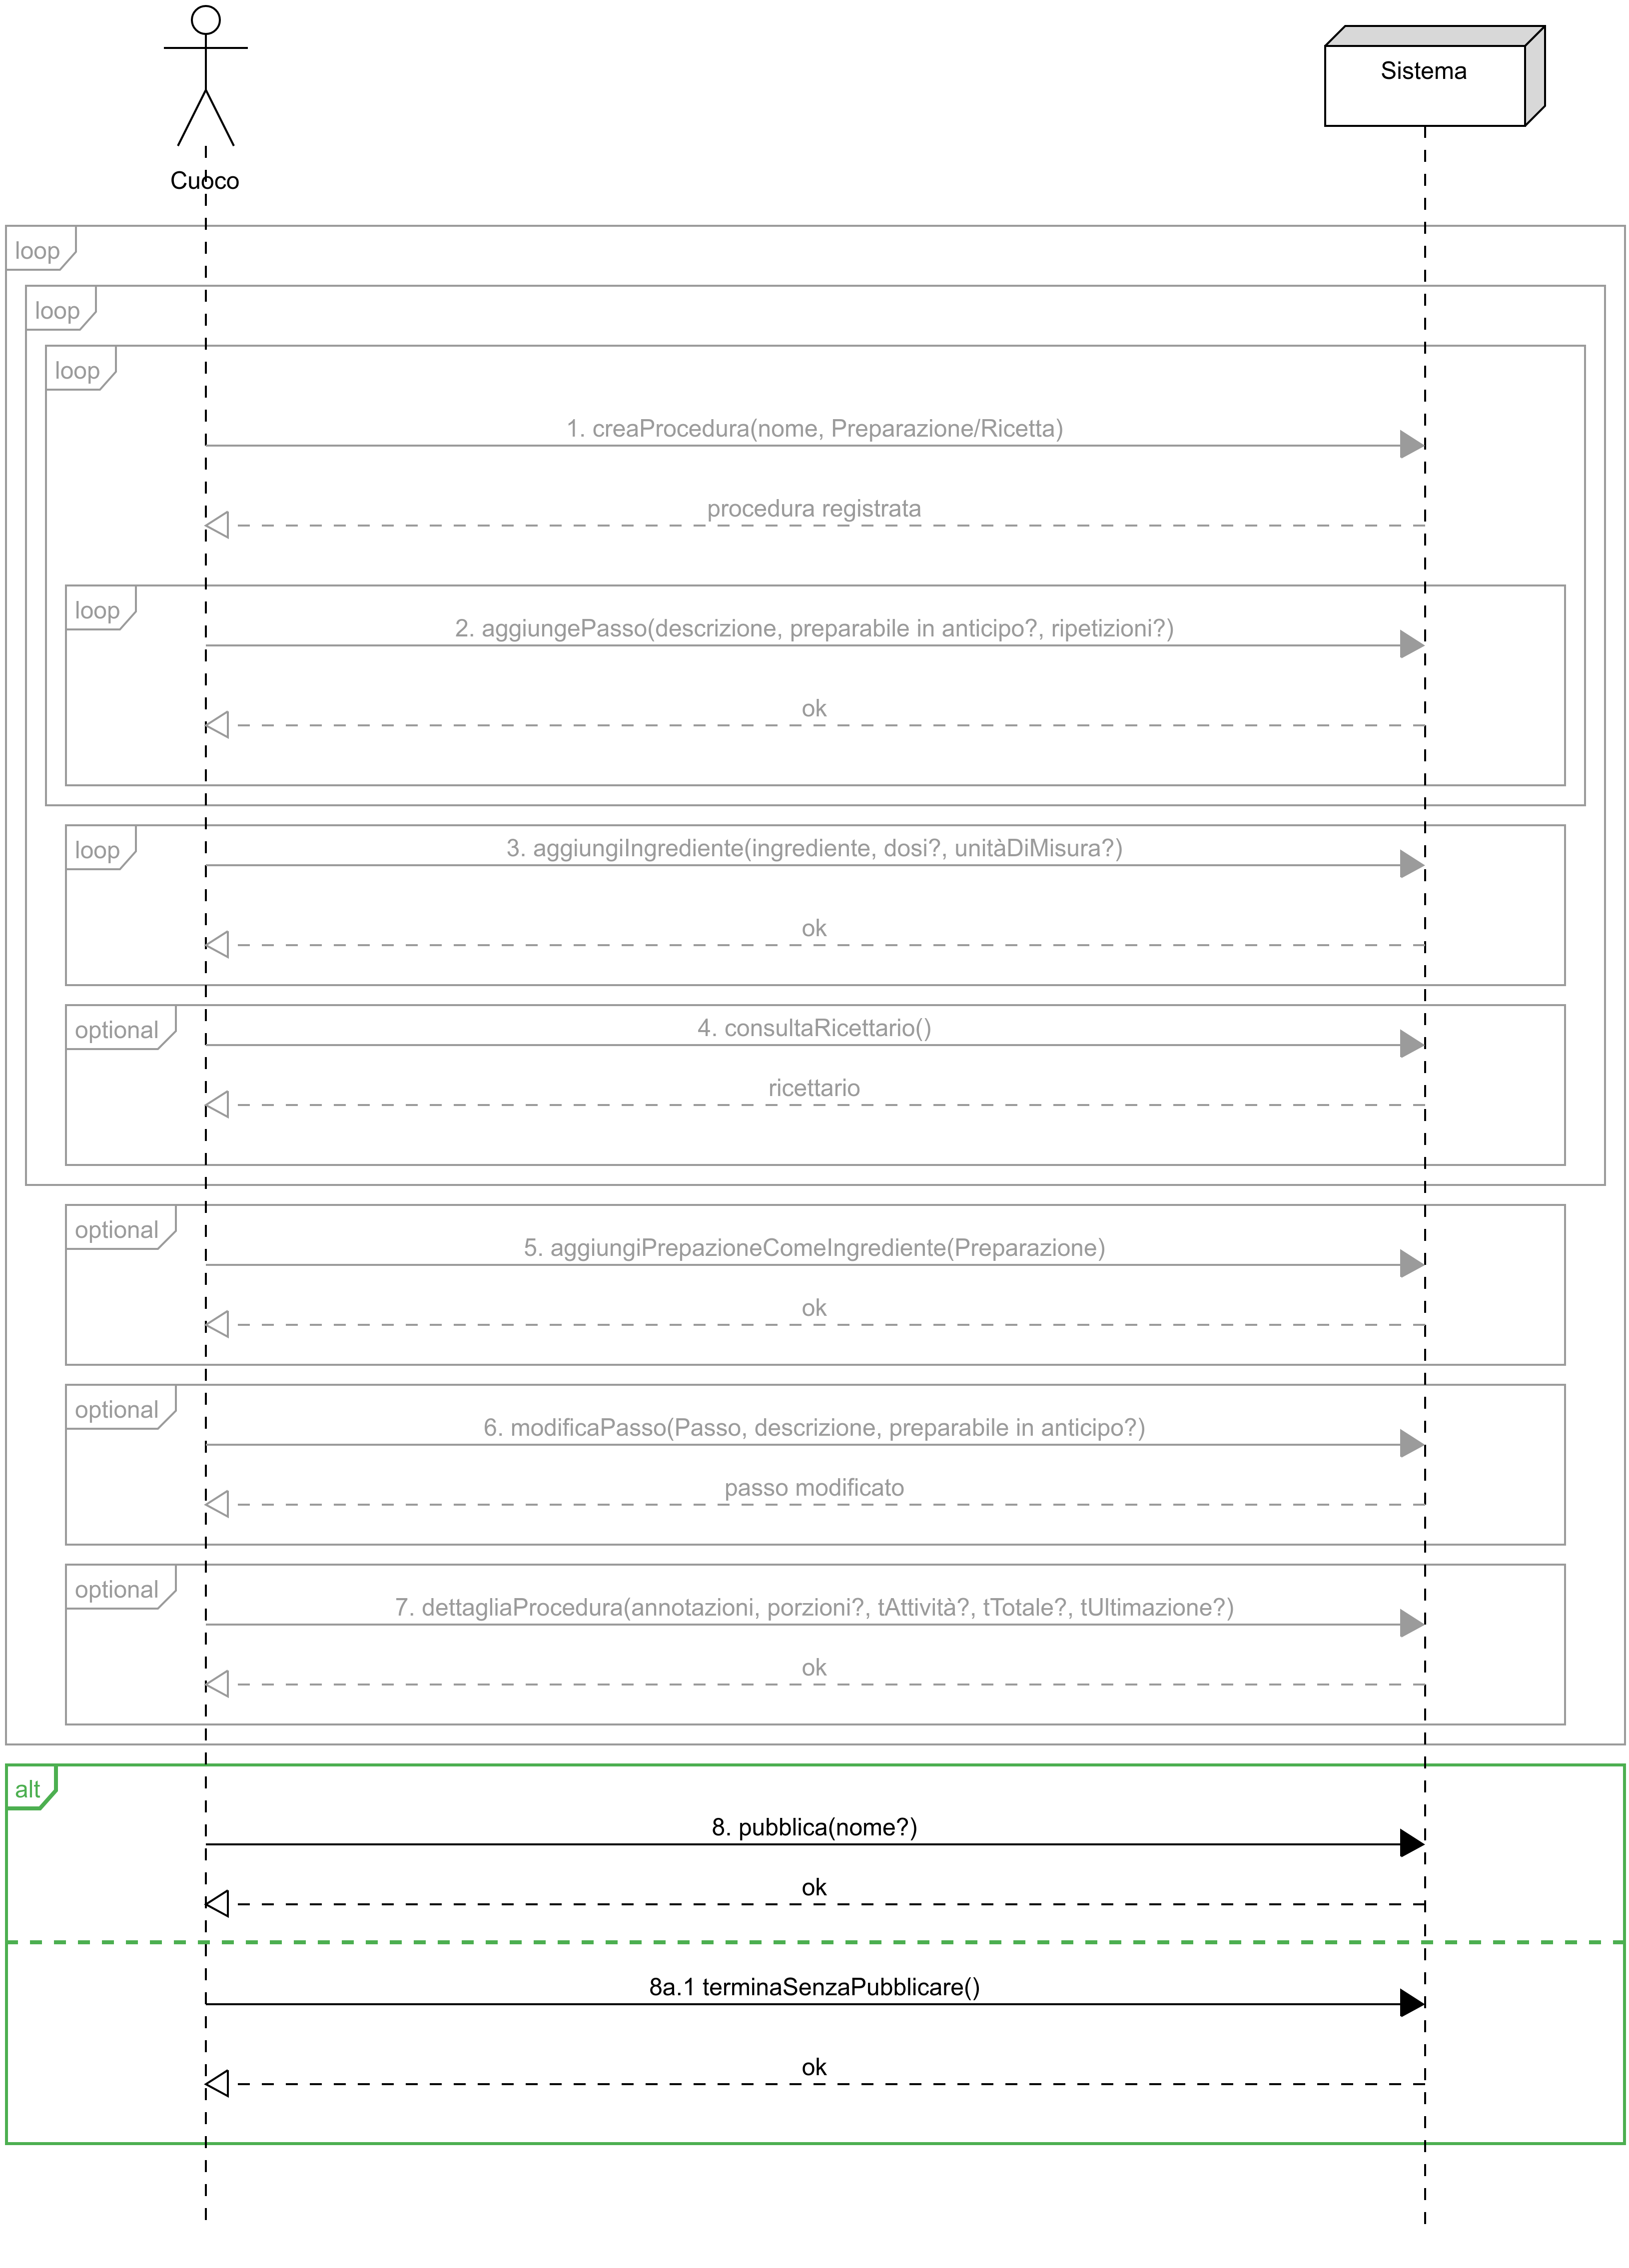
\includegraphics[max width=\textwidth, max height=190mm]{../resources/img/GRP/SSD/ext8.png}
\end{figure}
\RaggedRight

\chapter{Contratti delle Operazioni}
\textbf{Pre-condizione generale}{: l'utente è identificato come Chef }\textit{h}

\section[creaFoglioRiepilogativo]{\texorpdfstring{creaFoglioRiepilogativo(\myuline{servizio}: Servizio, \myuline{evento}: Evento)}}\label{h.n5k8dzisnnko}
\textbf{Pre-condizioni:}
\begin{itemize}[label=$-$, noitemsep]
	\item {allo Chef h }\textbf{è assegnato un }{evento che }{ }\textbf{prevede }{servizio}
\end{itemize}
\textbf{Post-condizioni:}
\begin{itemize}[label=$-$, noitemsep]
	\item {{[}\textbf{Se }{evento}{ è }\textbf{assegnato} a \textit{h} e \textbf{se}
		{non esiste un foglio riepilogativo che si }\textbf{riferisce} a \myuline{servizio}{]}}
	\begin{itemize}[label=$-$, noitemsep]
	\item {crea un'istanza }\textit{f}{ di FoglioRiepilogativo}
	\item \myuline{servizio}{ è }\textbf{riferito}{ a }\textit{f}
	\item {dato un Menu }\textit{m}{ usato in }\myuline{servizio}{:}
	\setlist{nolistsep}
		\begin{itemize}[label=$-$, noitemsep]
			\item {per ogni Procedura }\textit{pro}{ che }\textbf{serve per }\textit{m}
				  { è stata creata una istanza }\textit{a}{ di Assegnamento, }
				  \textit{a}\textbf{ riguarda }\textit{pro}{ e }\textit{f }\textbf{contiene}\textit{ a}
			\item \textit{a.completato}{ = no}
		\end{itemize}
	\end{itemize}
\end{itemize}

\subsection[scegliFoglioRiepilogativo]{\texorpdfstring{scegliFoglioRiepilogativo(\myuline{foglio}: FoglioRiepilogativo)}}\label{h.mtur9qf1842f}
\textbf{Pre-condizioni:}
\begin{itemize}[label=$-$, noitemsep]
	\item {il servizio }\textit{s}{, che si }\textbf{riferisce}{ a }\myuline{foglio}
		  {, }\textbf{prevede}{ un Evento e che è }\textbf{assegnato}{ a }\textit{h}
\end{itemize}
\textbf{Post-condizioni: }{-}

\section[aggiungiProcedura]{\texorpdfstring{aggiungiProcedura(\myuline{procedura}: Procedura)}}\label{h.dhz9dhqjmi4g}
\textbf{Pre-condizioni:}
\begin{itemize}[label=$-$, noitemsep]
	\item {È in corso la gestione dei compiti relativi a un Foglio Riepilogativo }\textit{f}
\end{itemize}
\textbf{Post-condizioni:}
\begin{itemize}[label=$-$, noitemsep]
	\item {è stata creata una istanza }\textit{a}{ di Assegnamento}
	\item \textit{a }\textbf{riguarda}{ la procedura }\textit{pro}
	\item \textit{f}{ }\textbf{contiene}{ }\textit{a}
\end{itemize}

\subsection[eliminaProcedura]{\texorpdfstring{eliminaProcedura(\myuline{procedura}: Procedura)}}\label{h.s4zynktv9olt}
\textbf{Pre-condizioni:}
\begin{itemize}[label=$-$, noitemsep]
	\item {È in corso la gestione dei compiti relativi a un Foglio Riepilogativo }\textit{f}
\end{itemize}
\textbf{Post-condizioni:}
\begin{itemize}[label=$-$, noitemsep]
	\item {per ogni }{Assegnamento}\textit{ a }\textbf{contenuto }{in }\textit{f}
		  { con }\textit{a}{ che }\textbf{riguarda }\myuline{procedura}{, le istanze }\textit{a}{ sono eliminate}
\end{itemize}

\section[riordinaElencoAssegnamenti]{\texorpdfstring{riordinaElencoAssegnamenti(\myuline{ordinamento})}}\label{h.rhtfki5g8w24}
\textbf{Pre-condizioni:}
\begin{itemize}[label=$-$, noitemsep]
	\item {È in corso la gestione dei compiti relativi a un Foglio Riepilogativo }\textit{f}
\end{itemize}
\textbf{Post-condizioni: }
\begin{itemize}[label=$-$, noitemsep]
	\item {l'associazione }\textbf{contiene }{tra }\textit{f}{ e gli Assegnamenti è modificata
		  in accordo a }\myuline{ordinamento}
\end{itemize}

\section[consultaTabelloneTurni]{\texorpdfstring{consultaTabelloneTurni()}}\label{h.w08r7f8npm2z}
\textbf{Pre-condizioni: }{-}\newline
\textbf{Post-condizioni: }{-}

\clearpage
\section[generaAssegnamento]{\texorpdfstring{generaAssegnamento(\myuline{assegnamento}{:
			  Assegnamento, }\myuline{turno}{?: Turno, }\myuline{cuoco}{?: Cuoco, }\myuline{stimaTempo}{?:
			  testo, }\myuline{dosi}{?: numero, }\myuline{continuazione}?: Assegnamento)}}\label{h.3umm3owhjhiq}
\textbf{Pre-condizioni:}
\begin{itemize}[label=$-$, noitemsep]
	\item {È in corso la gestione dei compiti relativi a un Foglio Riepilogativo }\textit{f}
	\item \textit{f}{ }\textbf{contiene}{ }\myuline{assegnamento}
	\item {Se }\myuline{continuazione}{ è specificato }\textit{f}{ }\textbf{contiene}{ }\myuline{continuazione}
	\item {il }\myuline{cuoco}{ ha dato disponibilità per }\myuline{turno} 
	\item {il }\myuline{turno}{ non si è ancora svolto}{ ed è dopo la data del }\myuline{servizio}{ riferito a }\textit{f}
\end{itemize}
\textbf{Post-condizioni:}
\begin{itemize}[label=$-$, noitemsep]
	\item {{[}}\textbf{Se}{ }\myuline{turno}{ è specificato{]} }
	\setlist{nolistsep}
	\begin{itemize}[label=$-$, noitemsep]
		\item {[}\textbf{Se esiste }{un }\myuline{cuoco}{ c che } \textbf{esegue }\myuline{assegnamento}{ e }\textbf{Se }\myuline{assegnamento.tempoStimato}{ è definito}{]}
		\setlist{nolistsep}
		\begin{itemize}[label=$-$, noitemsep]
			\item {{[}}\textbf{Se}{ esiste una istanza} \textit{ct} {Cuoco in turno che associa }\textit{cuoco} e \textit{turno} {e Se {l'istanza }\textit{ct}{ Cuoco in Turno che associa }\textit{c} e il turno \textit{t} dove viene \textbf{svolto} \myuline{assegnamento} ha \\\textit{ct.tempoDisponibile} $<$ \myuline{assegnamento.tempoStimato}}{]}
				  {l'istanza }\textit{ct} ha \textit{ct.tempoDisponibile} $=$ \textit{ct.tempoDisponibile} $-$ \myuline{assegnamento.tempoStimato} 
			\item \myuline{assegnamento}{ si }\textbf{svolge}{ in }\myuline{turno}
		\end{itemize}
    \end{itemize}
	\item {{[}}\textbf{Se}{ }\myuline{stimaTempo}{ è specificato{]} }                       
	\setlist{nolistsep}
	\begin{itemize}[label=$-$, noitemsep]
		\item {[}\textbf{Se esiste }{un }\myuline{cuoco}{ c che } \textbf{esegue }\myuline{assegnamento}{ e }\textbf{Se esiste}{un }\myuline{turno}{ t dove si } \textbf{svolge }\myuline{assegnamento}{]}
		\setlist{nolistsep}
		\begin{itemize}[label=$-$, noitemsep]
			\item {{[}}\textbf{Se}{ esiste una istanza} \textit{ct} {Cuoco in turno che associa }\textit{cuoco} e \textit{turno} {e Se {l'istanza }\textit{ct}{ Cuoco in Turno che associa }\textit{c} e il turno \textit{t} dove viene \textbf{svolto} \myuline{assegnamento} ha \\\textit{ct.tempoDisponibile} $<$ \myuline{stimaTempo}}{]}
			      {l'istanza }\textit{ct} ha \textit{ct.tempoDisponibile} $=$ \textit{ct.tempoDisponibile} $-$ \myuline{stimaTempo} 
			\item \myuline{assegnamento.tempoStimato} $=$ \myuline{stimaTempo}
		\end{itemize}
    \end{itemize}
	\item {{[}}\textbf{Se }\myuline{cuoco}{ è specificato{]}}
	\setlist{nolistsep}
	\begin{itemize}[label=$-$, noitemsep]
		\item {[}\textbf{Se esiste }{un }\myuline{turno}{ t dove si} \textbf{svolge }\myuline{assegnamento}{ e }\textbf{Se }\myuline{assegnamento.tempoStimato}{ è definito}{]}
		\setlist{nolistsep}
		\begin{itemize}[label=$-$, noitemsep]
			\item {{[}}\textbf{Se}{ esiste una istanza} \textit{ct} {Cuoco in turno che associa }\textit{cuoco} e \textit{turno} {e Se {l'istanza }\textit{ct}{ Cuoco in Turno che associa }\textit{c} e il turno \textit{t} dove viene \textbf{svolto} \myuline{assegnamento} ha \\\textit{ct.tempoDisponibile} $<$ \myuline{stimaTempo}}{]}
			  	  {l'istanza }\textit{ct} ha \textit{ct.tempoDisponibile} $=$ \textit{ct.tempoDisponibile} $-$ \myuline{stimaTempo} 
			\item \myuline{assegnamento}{ è }\textbf{eseguito}{ da }\myuline{cuoco}
		\end{itemize}
	\end{itemize}
	\item {{[}}\textbf{Se }\myuline{continuazione}{ è specificato{]}} \myuline{assegnamento}{ è }\textbf{continuazione}{ di }\myuline{continuazione}
	\item {{[}}\textbf{Se }\myuline{dosi}{ è specificato{]}} \myuline{assegnamento.quantità} $=$ \myuline{dosi}
\end{itemize}

\clearpage
\subsection[specificaAssegnamentoCompletato]{\texorpdfstring{specificaAssegnamentoCompletato(\myuline{assegnamento}: Assegnamento)}}\label{h.c49s37d45gzr}
\textbf{Pre-condizioni: }
\begin{itemize}[label=$-$, noitemsep]
	\item {È in corso la gestione dei compiti relativi a un Foglio Riepilogativo }\textit{f}
	\item \textit{f}{ }\textbf{contiene}{ }\myuline{assegnamento}
\end{itemize}
\textbf{Post-condizioni: }
\begin{itemize}[label=$-$, noitemsep]
	\item \myuline{assegnamento.completato}{ = sì}
\end{itemize}

\subsection[eliminaAssegnamento]{\texorpdfstring{eliminaAssegnamento(\myuline{assegnamento}: Assegnamento)}}\label{h.g9i7rk2xvxb7}
\textbf{Pre-condizioni:  }
\begin{itemize}[label=$-$, noitemsep]
	\item {È in corso la gestione dei compiti relativi a un Foglio Riepilogativo }\textit{f}
	\item \textit{f}{ }\textbf{contiene}{ }\myuline{assegnamento}
\end{itemize}
\textbf{Post-condizioni:}
\begin{itemize}[label=$-$, noitemsep]
	\item
		  {{[}\textbf{Se esiste} un un assegnamento }\textit{a1}{ che è }\textbf{continuato }{da
		  }\myuline{assegnamento}{ ed esiste un assegnamento }\textit{a2}{ che è }\textbf{continuazione
		  }{di }\myuline{assegnamento}{]} \textit{a2}{ è }\textbf{continuazione }{di }\textit{a1}
	\item \myuline{assegnamento} è stato eliminato
	\item {[}\textbf{Se esiste }{un }\myuline{cuoco}{ c che } \textbf{esegue }\myuline{assegnamento}{, }
	\textbf{Se esiste}{ un Turno }\textit{t}{ }{tale che}{ }\myuline{assegnamento}{ è}\textbf{svolto }{in }\textit{t}
	{ e }\textbf{Se }\myuline{assegnamento.tempoStimato}{ è definito}{]}
	{l'istanza }\textit{ct}{ Cuoco in Turno che associa }\textit{c} e il turno \textit{t} dove viene \textbf{svolto} \myuline{assegnamento} ha \\\textit{ct.tempoDisponibile} $=$ \textit{ct.tempoDisponibile} $+$ \myuline{assegnamento.tempoStimato}
\end{itemize}


\addtocontents{toc}{\protect\newpage}\part{Progettazione}
\uselandscape
\chapter{Domain Class Diagram}
\begin{figure}[H]
  \centering\includegraphics[max width=\textwidth, max height=143mm]{../resources/img/Domain Class Diagram.png}
\end{figure}

\chapter{Design Sequence Diagrams}
\begingroup\centering
\renewcommand{\thesection}{2}
\section{addSimpleCookingStep}
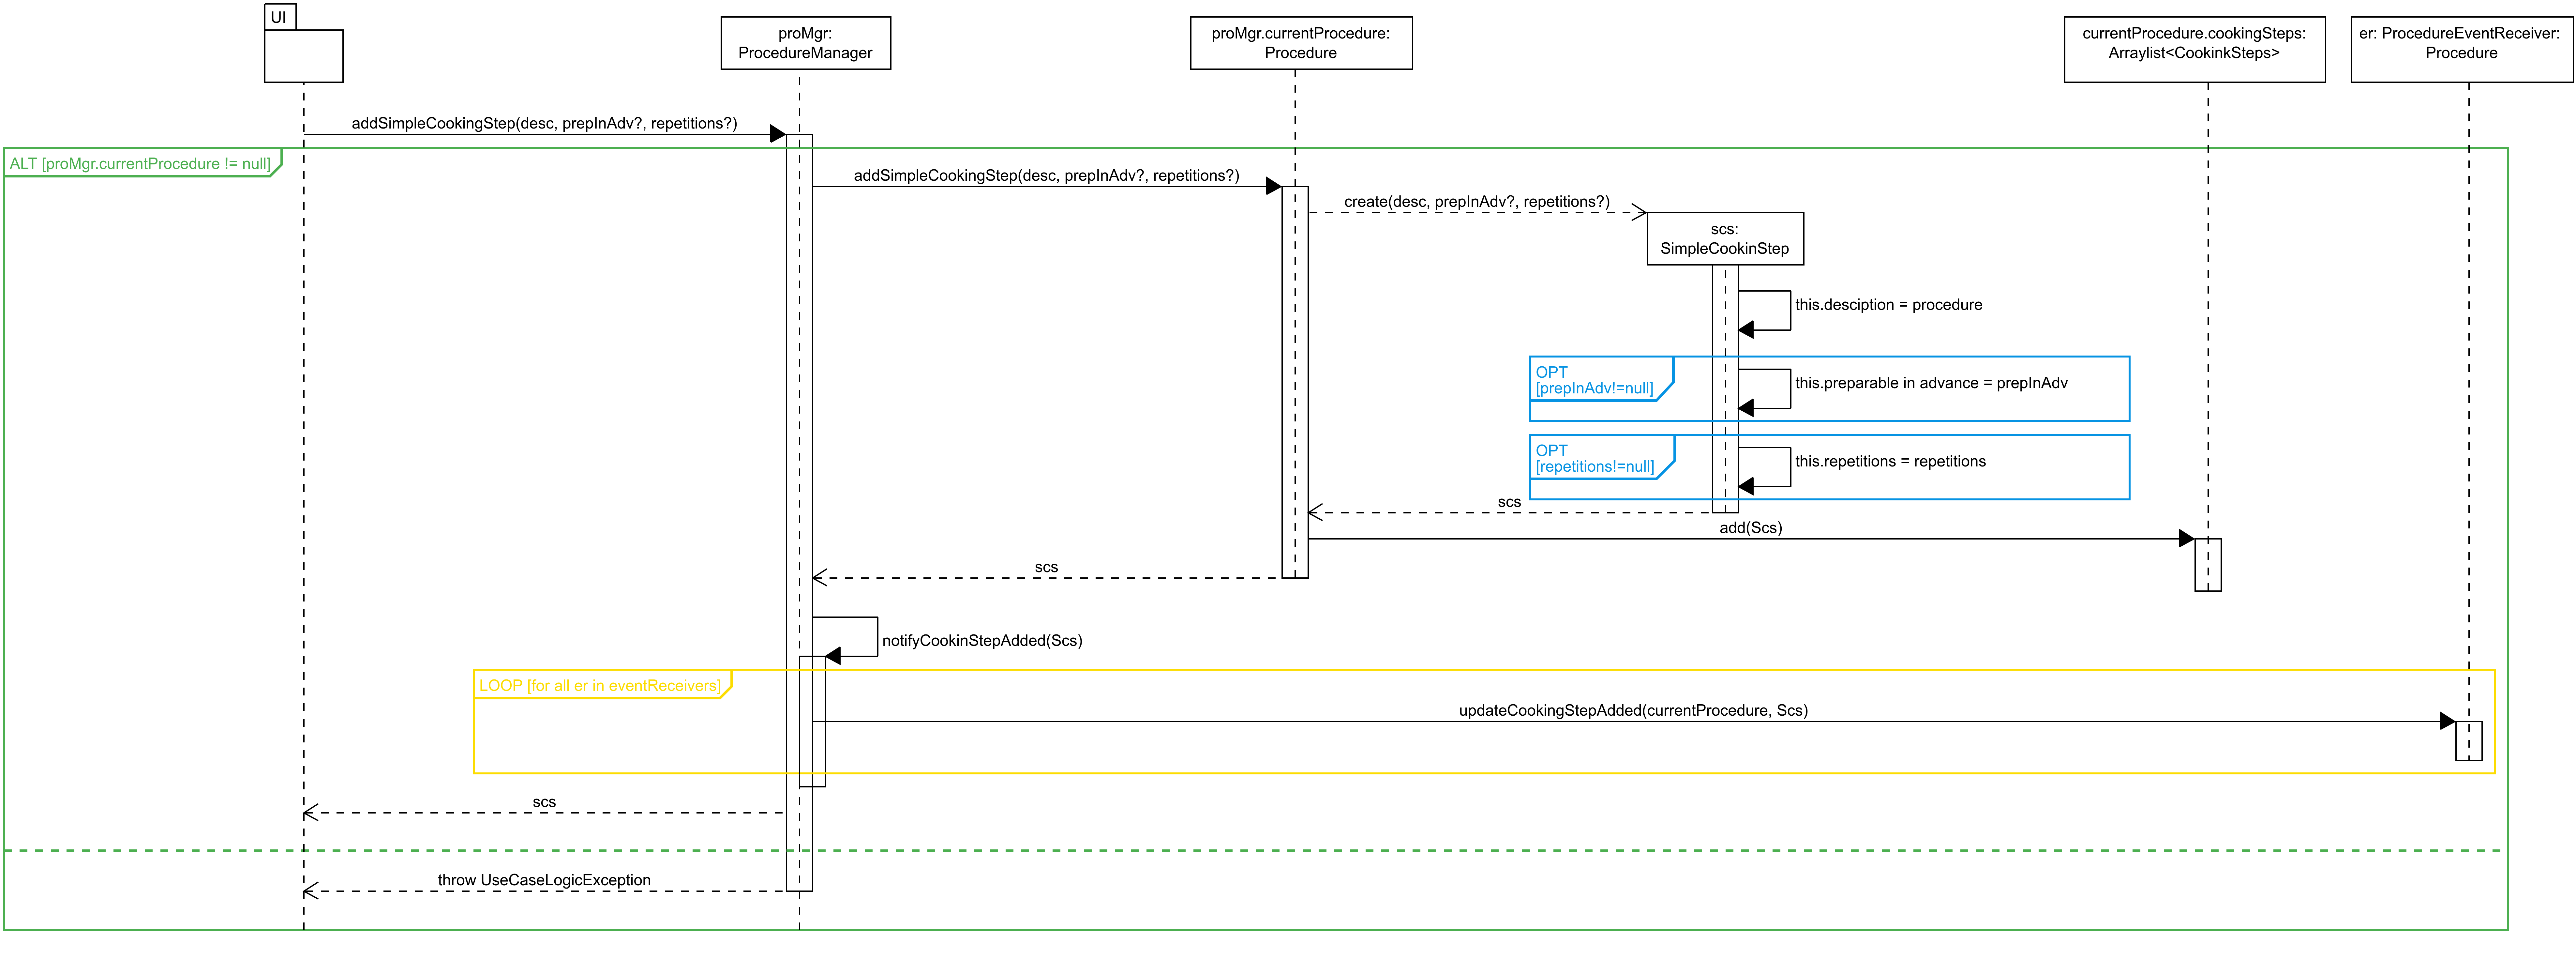
\includegraphics[max width=\textwidth, max height=158mm]{../resources/img/GRP/DSD/op2.png}

\subsection{addGroupingCookingStep}
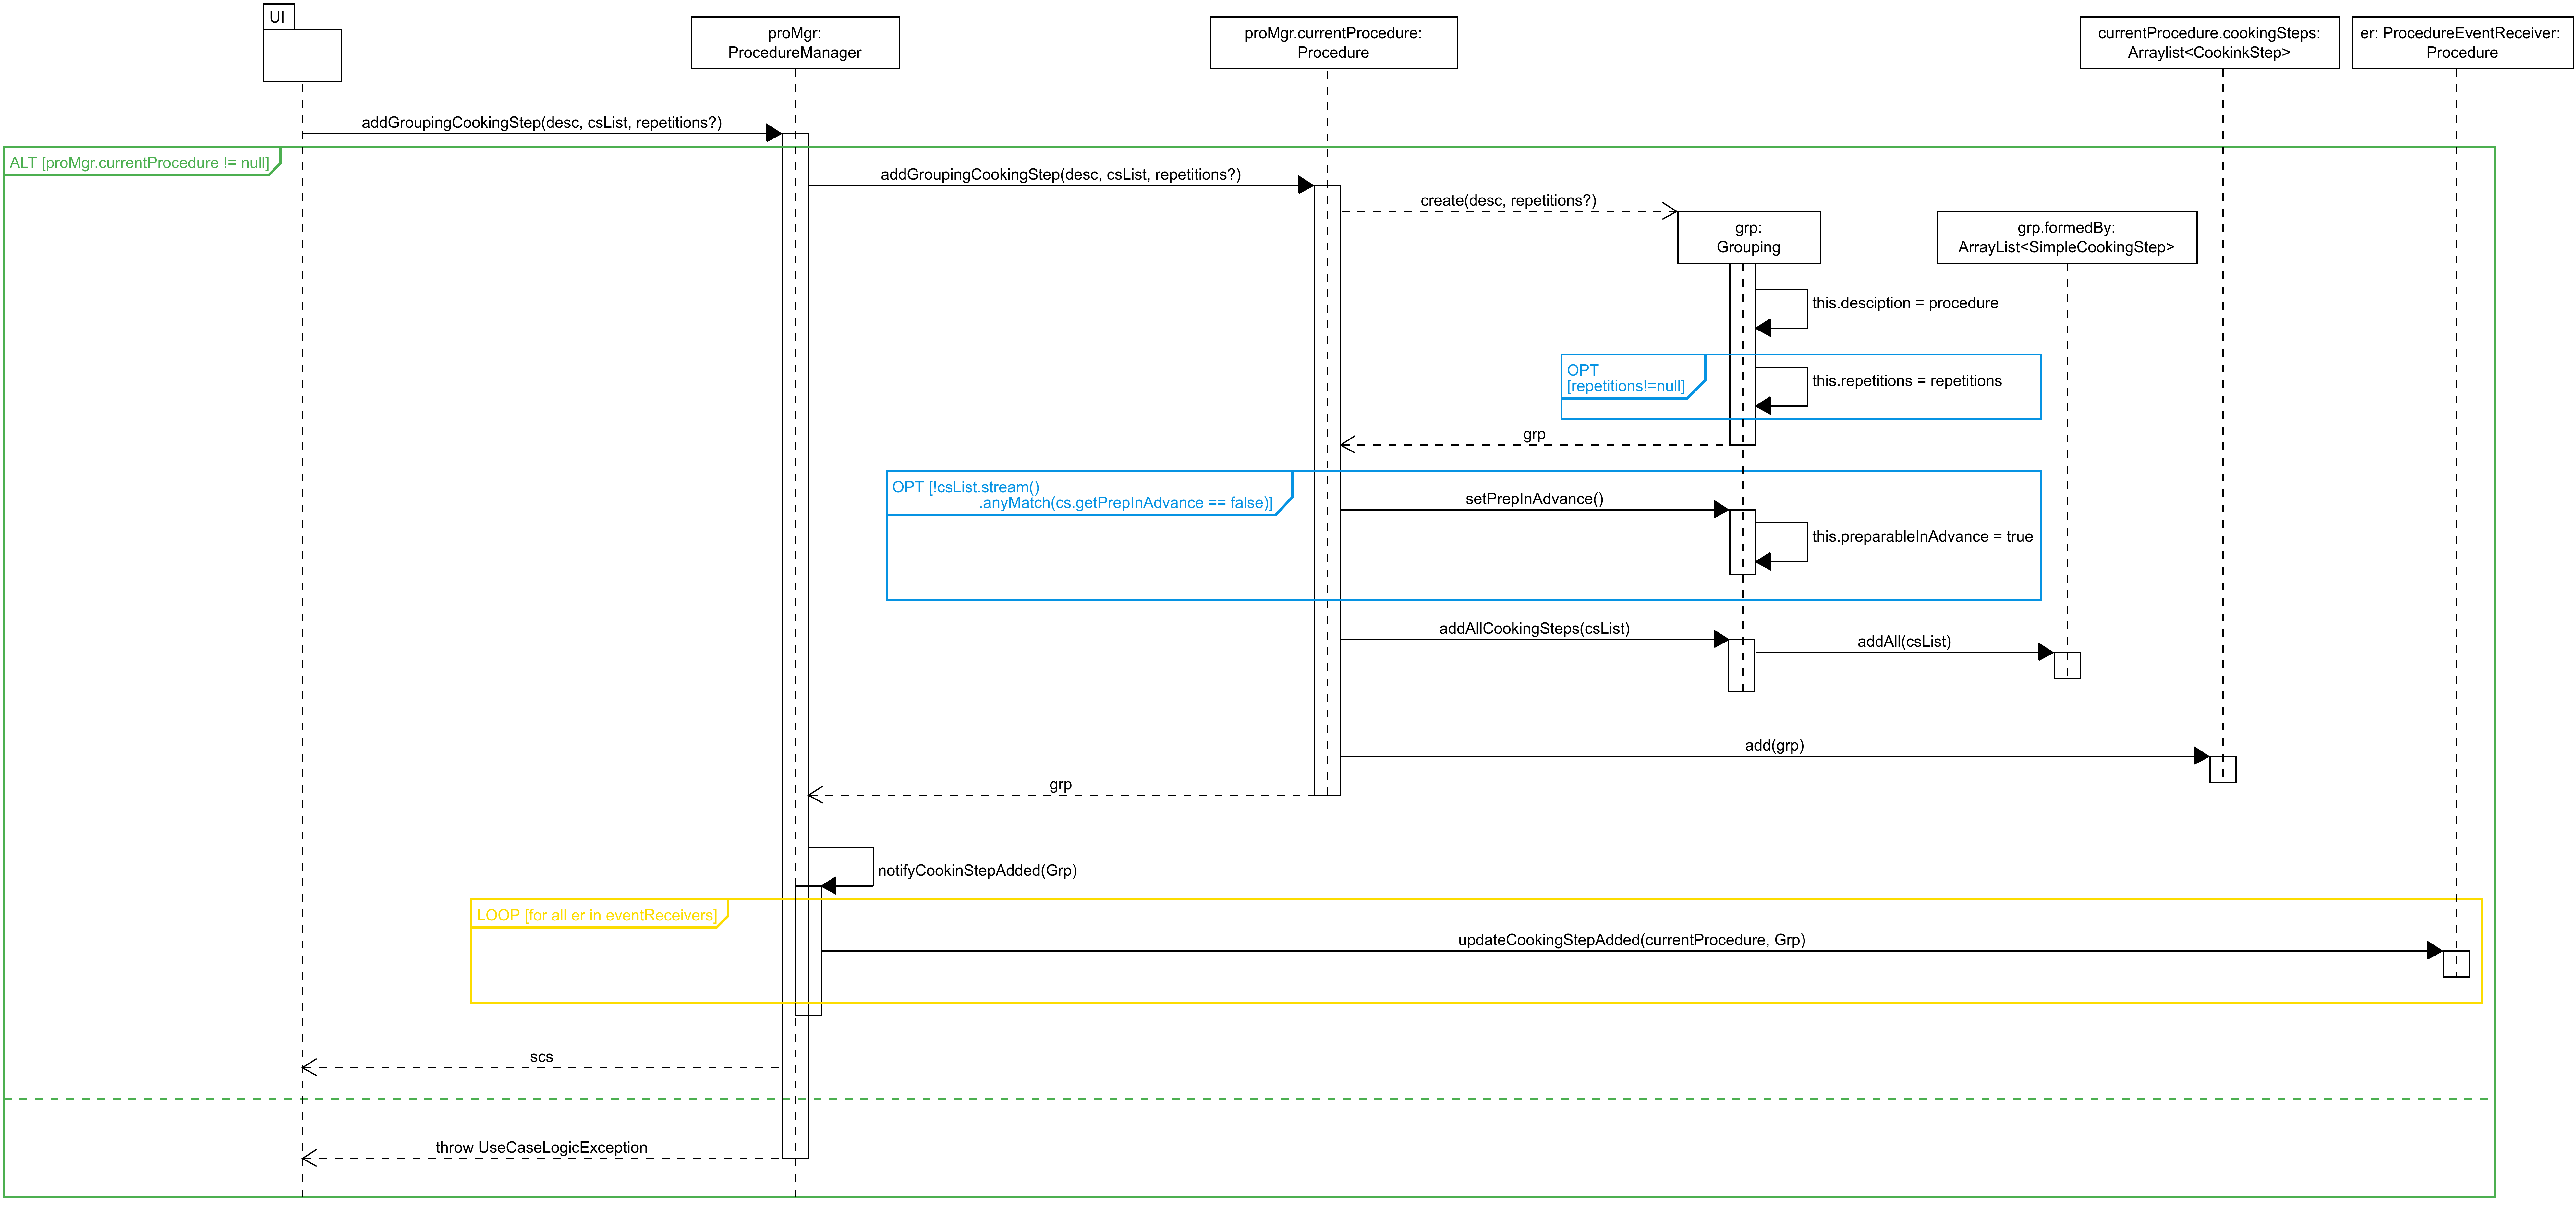
\includegraphics[max width=\textwidth, max height=190mm]{../resources/img/GRP/DSD/op2a.png}
\endgroup

\begingroup\centering
\renewcommand{\thesection}{3}
\section{addIngredient}
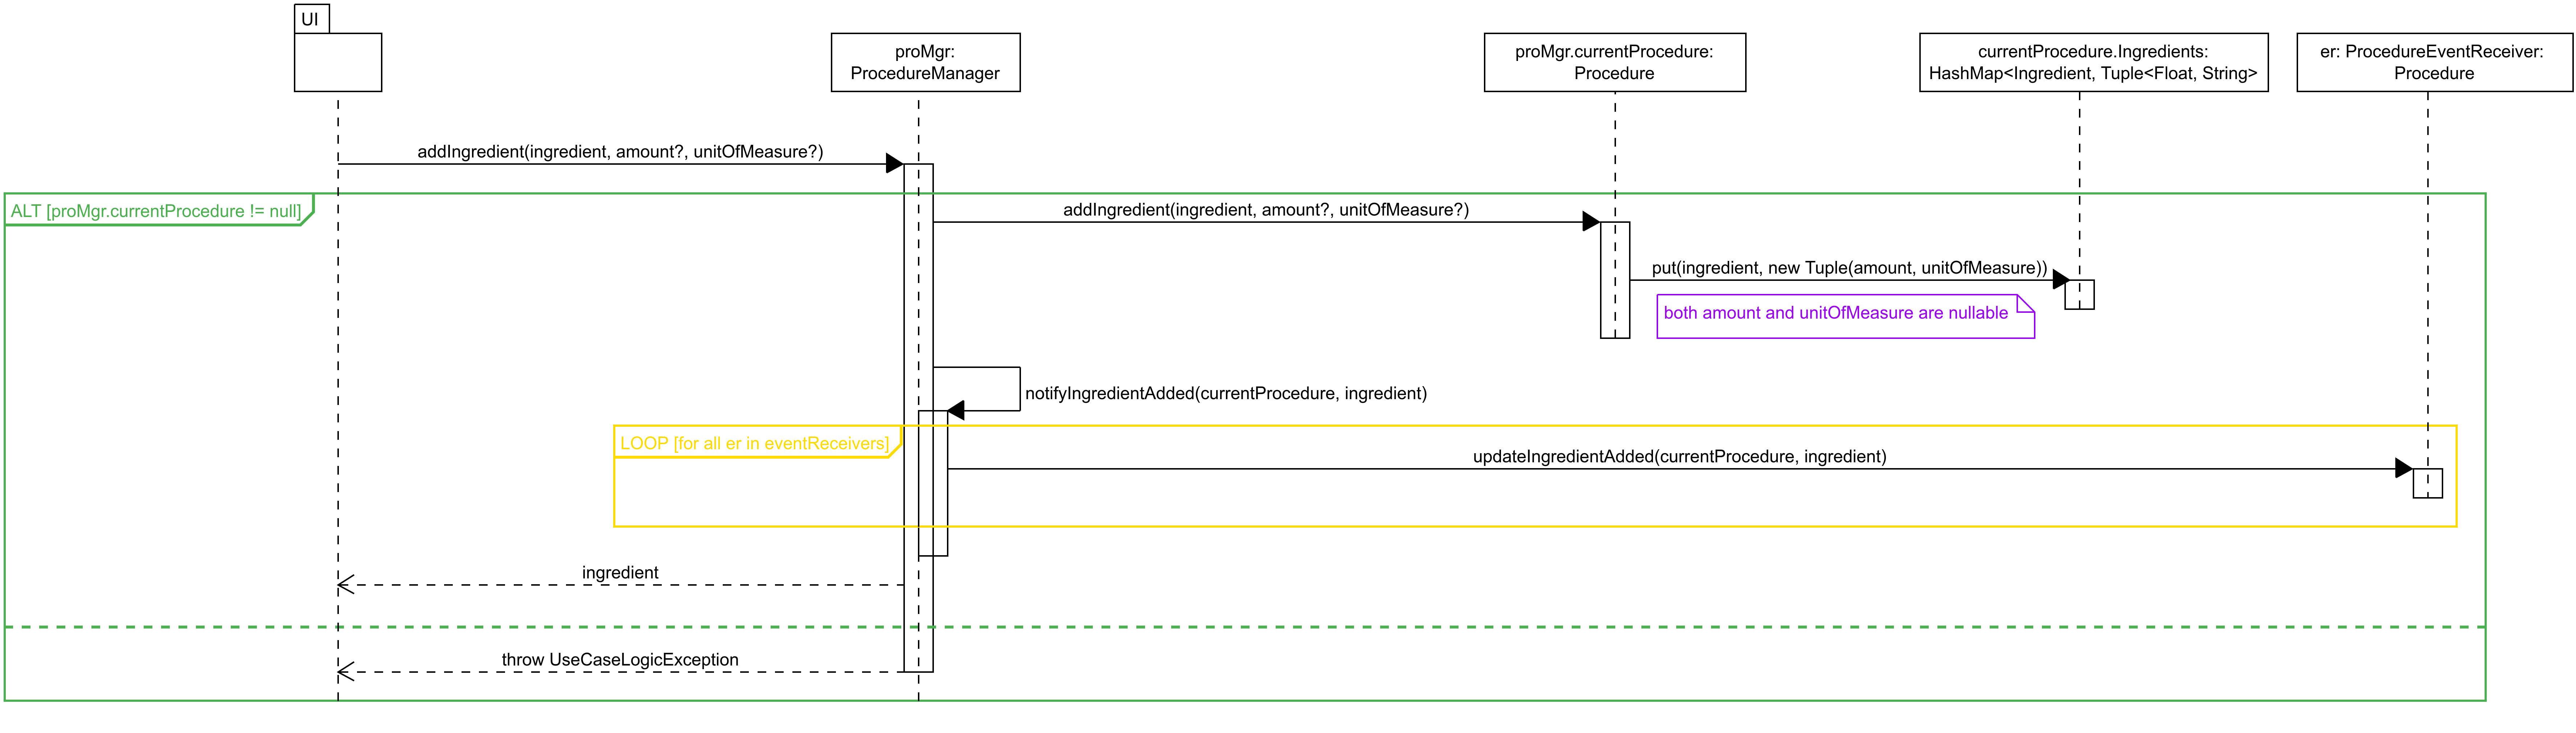
\includegraphics[max width=\textwidth, max height=190mm]{../resources/img/GRP/DSD/op3.png}
\endgroup

\begingroup\centering
\renewcommand{\thesection}{5}
\section{addPreparationAsIngredient}
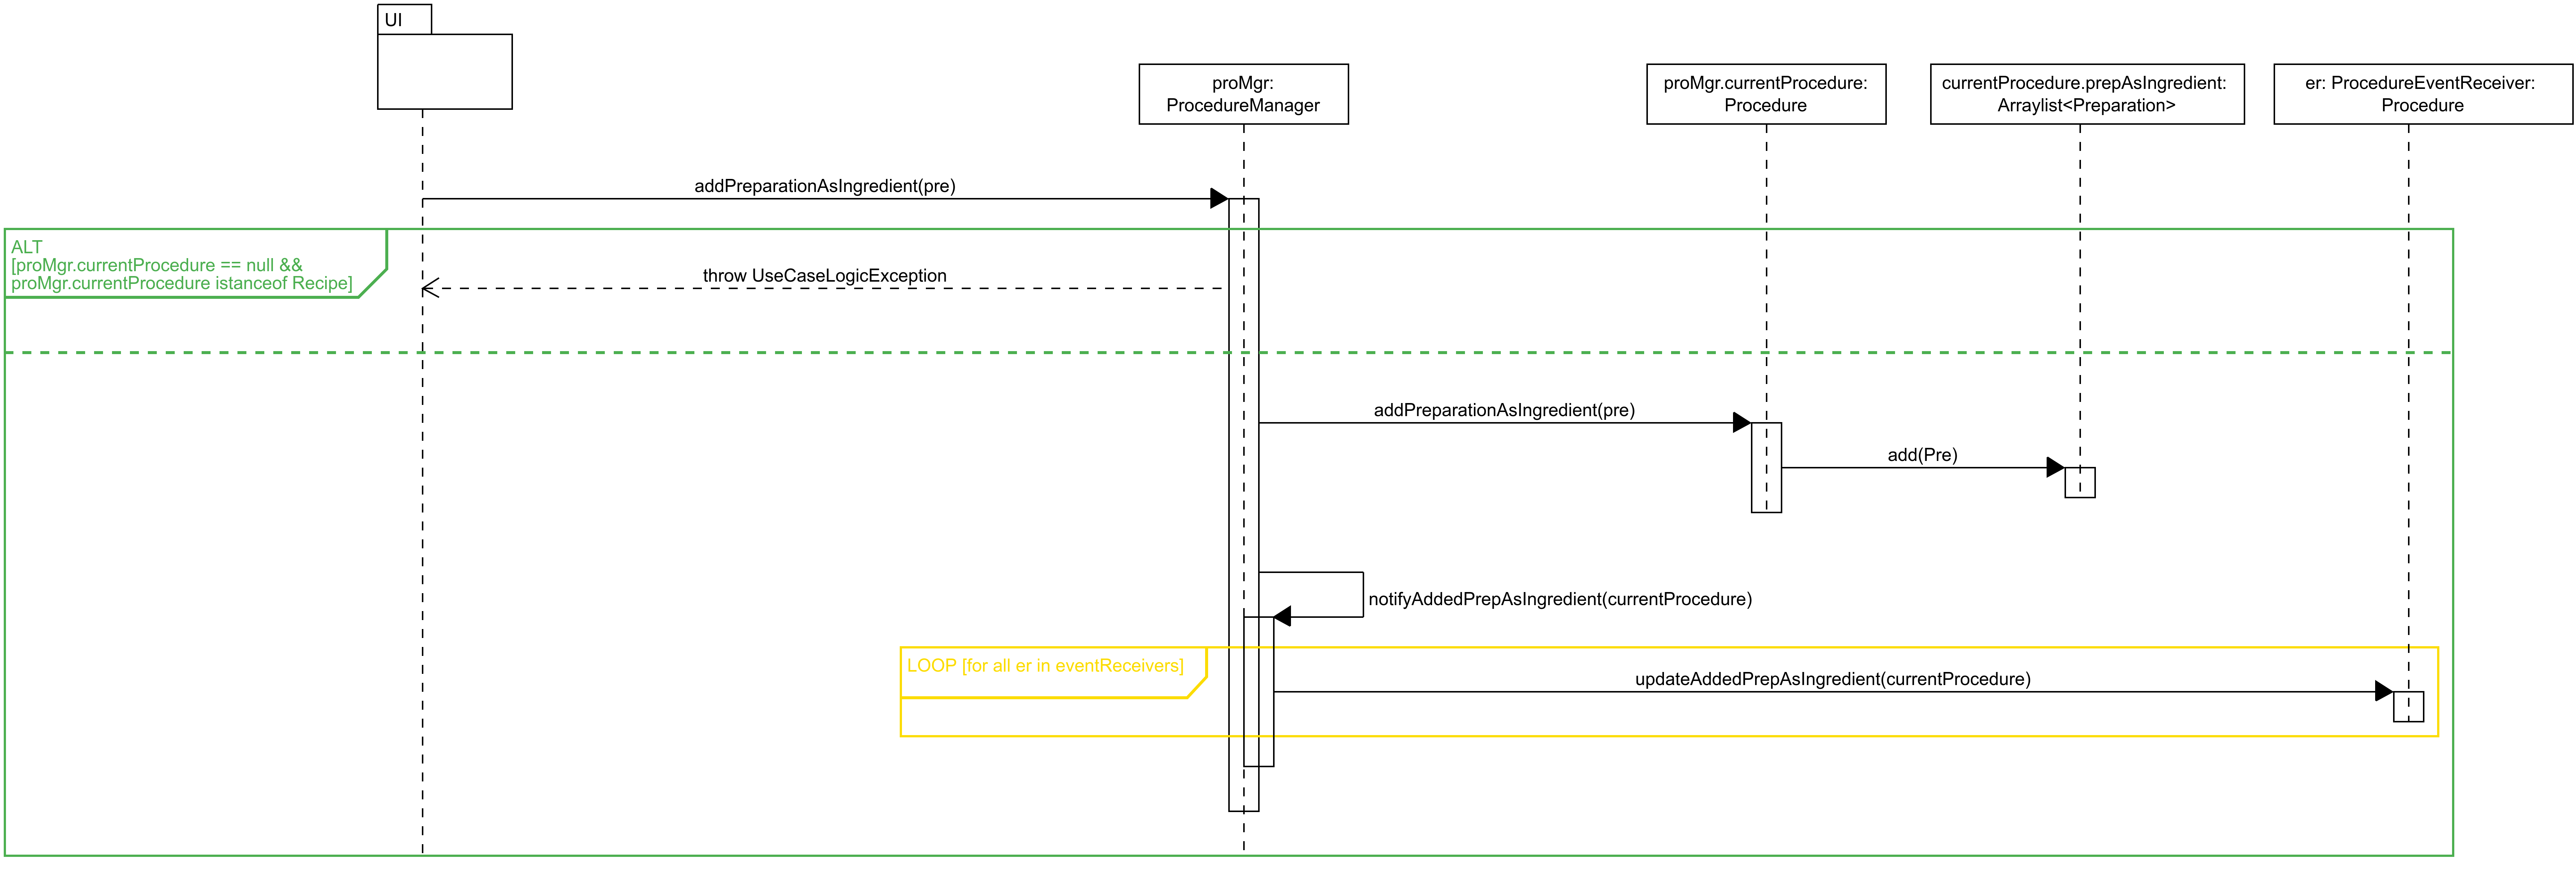
\includegraphics[max width=\textwidth, max height=190mm]{../resources/img/GRP/DSD/op5.png}
\endgroup

\begingroup\centering
\renewcommand{\thesection}{7}
\section{detailProcedure}
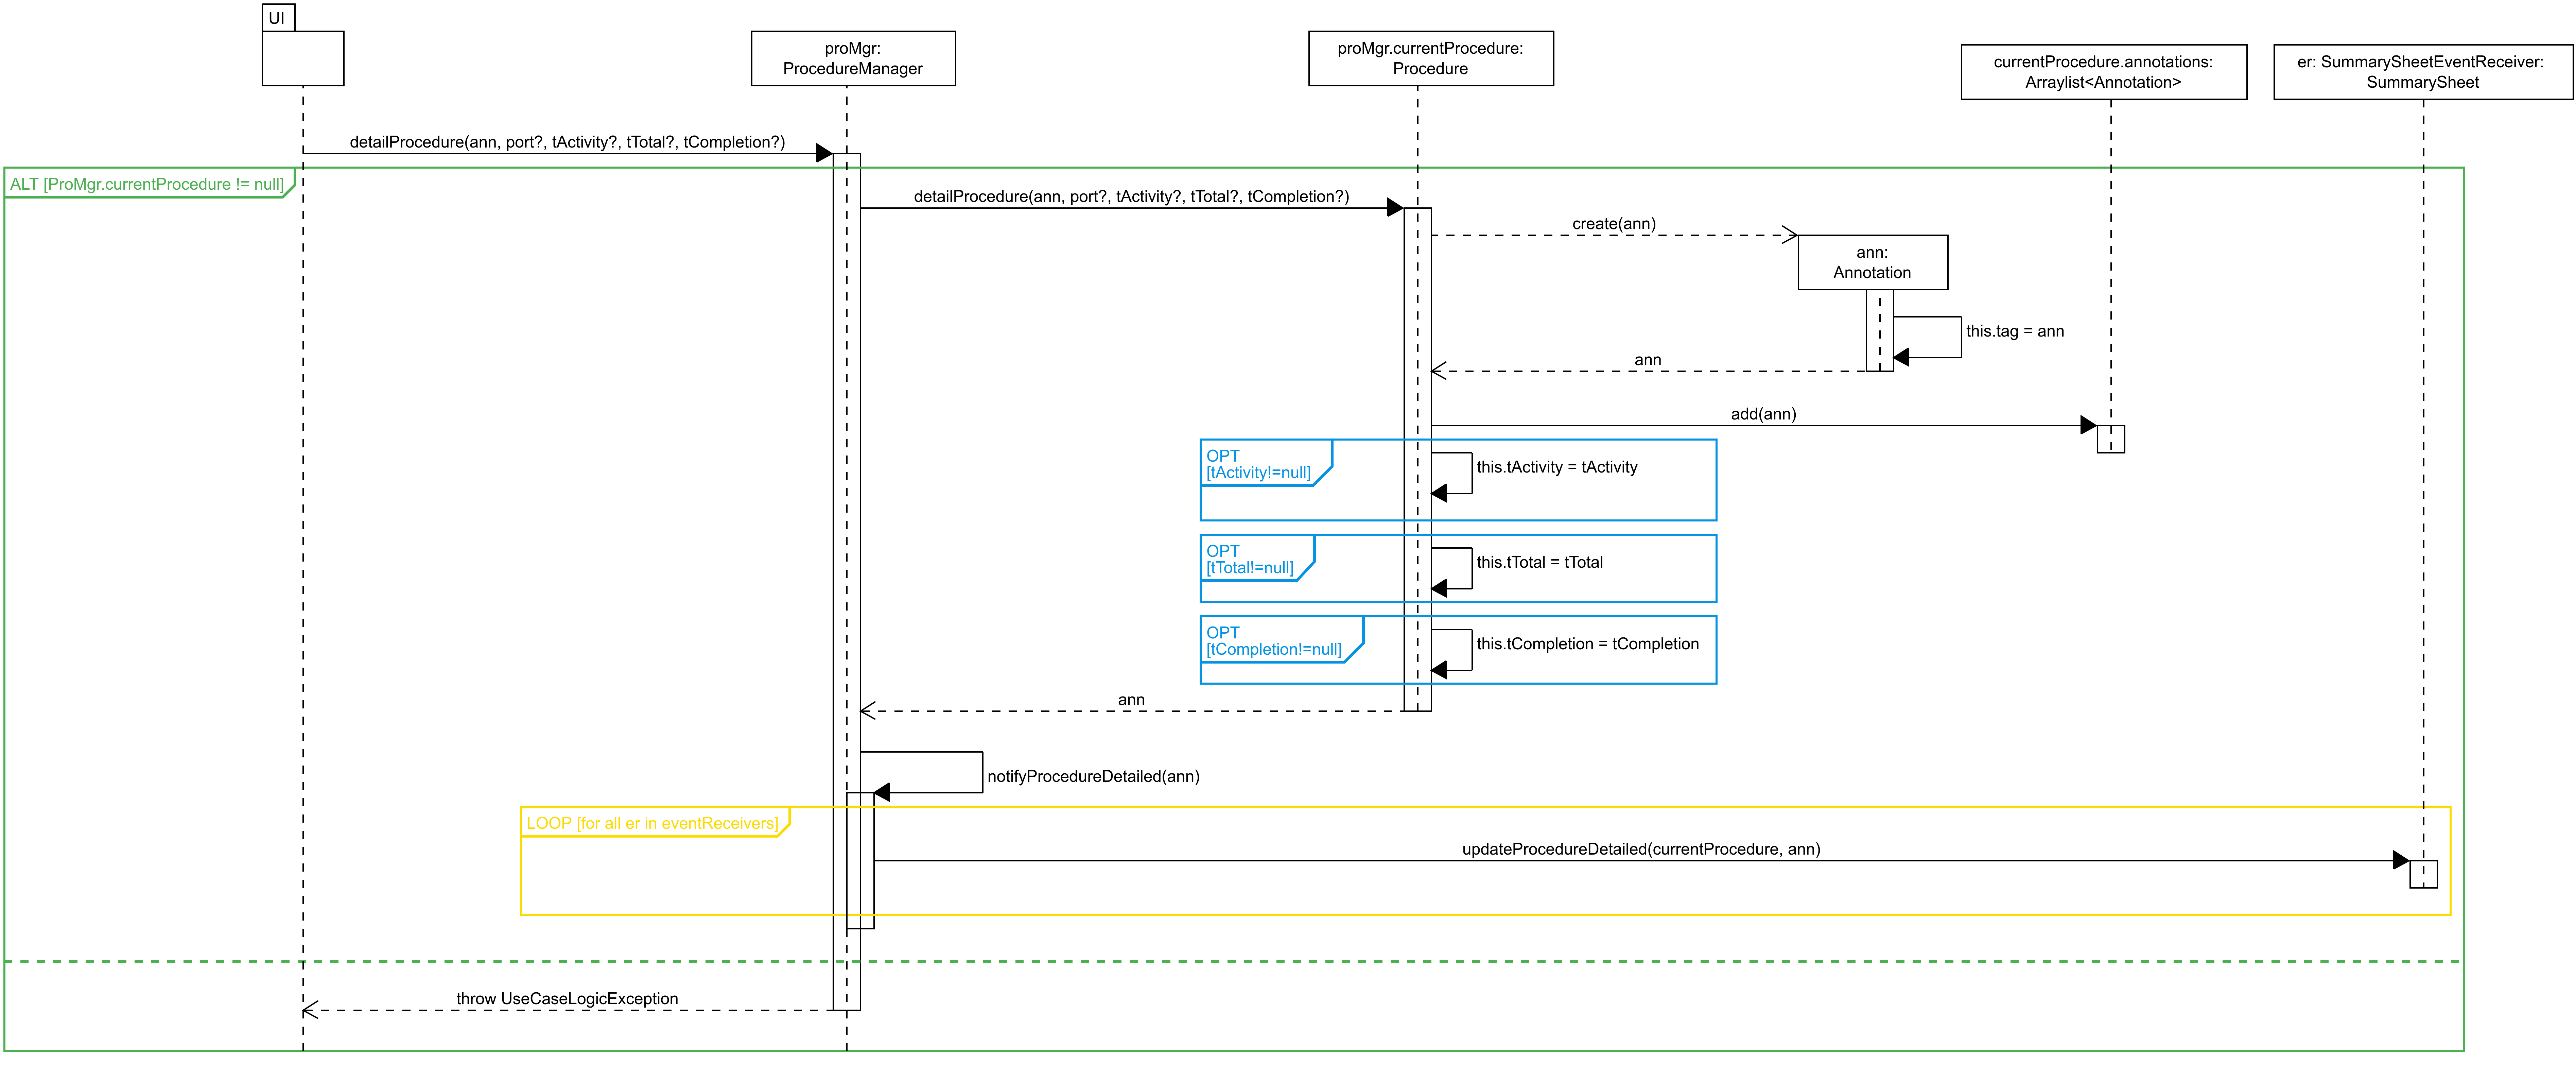
\includegraphics[max width=\textwidth, max height=190mm]{../resources/img/GRP/DSD/op7.png}

\begingroup\centering
\renewcommand{\thesubsection}{\thesection.d.1}
\subsection{extrapolateProcedure}
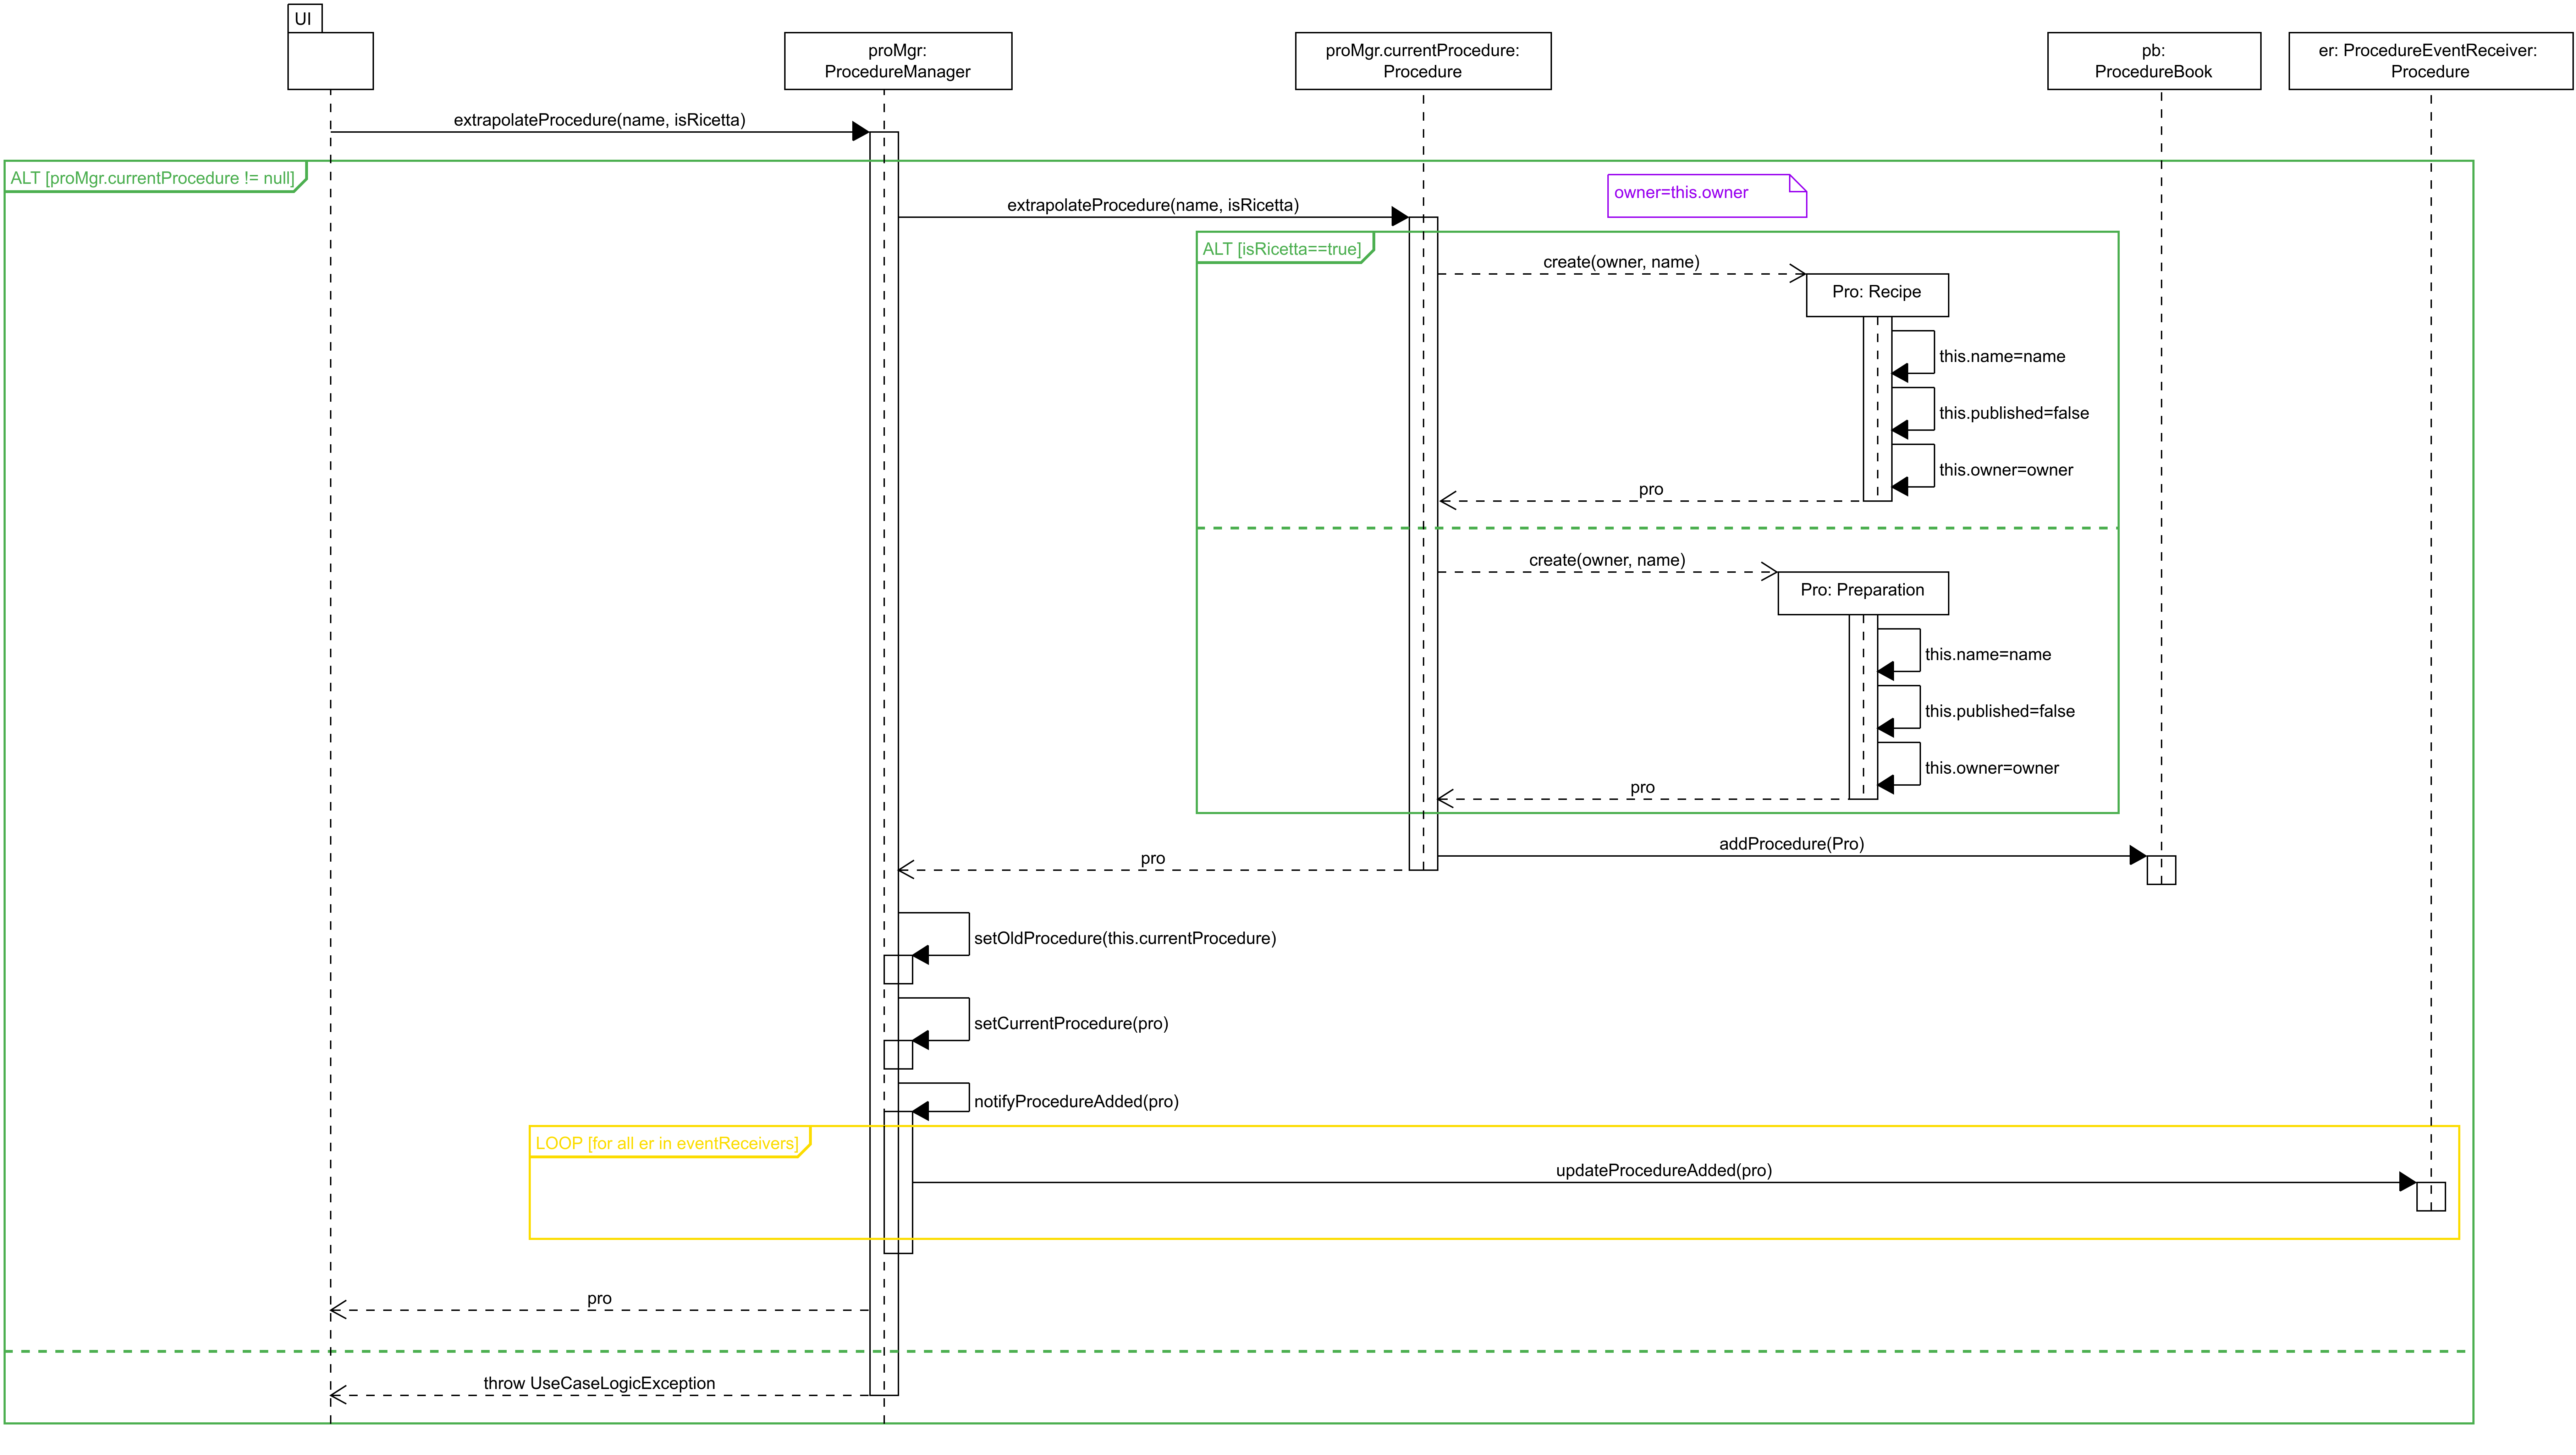
\includegraphics[max width=\textwidth, max height=190mm]{../resources/img/GRP/DSD/op7d.png}
\endgroup
\endgroup

\end{document}